% This must be in the first 5 lines to tell arXiv to use pdfLaTeX, which is strongly recommended.
\pdfoutput=1
% In particular, the hyperref package requires pdfLaTeX in order to break URLs across lines.

\documentclass[11pt]{article}

% Change "review" to "final" to generate the final (sometimes called camera-ready) version.
% Change to "preprint" to generate a non-anonymous version with page numbers.
\usepackage[preprint]{acl}

% Standard package includes
\usepackage{times}
\usepackage{latexsym}

% For proper rendering and hyphenation of words containing Latin characters (including in bib files)
\usepackage[T1]{fontenc}
% For Vietnamese characters
% \usepackage[T5]{fontenc}
% See https://www.latex-project.org/help/documentation/encguide.pdf for other character sets

% This assumes your files are encoded as UTF8
\usepackage[utf8]{inputenc}

% This is not strictly necessary, and may be commented out,
% but it will improve the layout of the manuscript,
% and will typically save some space.
\usepackage{microtype}

% This is also not strictly necessary, and may be commented out.
% However, it will improve the aesthetics of text in
% the typewriter font.
\usepackage{inconsolata}

%Including images in your LaTeX document requires adding
%additional package(s)
\usepackage{graphicx}
\usepackage{url}
\usepackage{enumitem}
\usepackage{booktabs}
\usepackage{makecell}
\usepackage{multirow}
\usepackage{algorithm}
\usepackage{algpseudocode}
\usepackage{amssymb}
\usepackage{amsmath}
\usepackage{pifont}
\usepackage[most]{tcolorbox}
\usepackage{soul}
\usepackage{xcolor}
\usepackage{ulem}
% \usepackage{minted}

\usepackage{pgfplotstable}
\usepackage{subfigure}
\usepackage{pgfplots}
\usepackage{tikz}
\usetikzlibrary{arrows.meta}
\usetikzlibrary{decorations}
\usetikzlibrary{pgfplots.groupplots}
\usepgfplotslibrary{fillbetween}
\usetikzlibrary{shapes.multipart}
\usetikzlibrary{shapes.geometric}

\definecolor{ugreen}{cmyk}{1,0,1,0.498}
\definecolor{lyyblue}{cmyk}{0.8278,0.3333,0,0.2941}
\definecolor{lyygreen}{cmyk}{0.6813,0,0.725,0.3725}
\definecolor{lyyred}{cmyk}{0,0.8855,0.8767,0.1098}
\definecolor{dblue}{cmyk}{1,0.5487,0,0.5569}
\definecolor{royalblue}{HTML}{4169e1}

\definecolor{myred}{HTML}{E33222}

\newcommand{\cmark}{\ding{52}}%
\newcommand{\xmark}{\ding{56}}%

\definecolor{gr}{RGB}{0, 146, 0}
\newcommand{\gr}[1]{\textcolor{gr}{#1}}
\newcommand{\red}[1]{\textcolor{myred}{#1}}
\newcommand{\purp}[1]{\textcolor{purple}{#1}}
\newcommand{\org}[1]{\textcolor{orange}{#1}}
\newcommand{\blue}[1]{\textcolor{blue}{#1}}
\newcommand{\teal}[1]{\textcolor{teal}{#1}}
\newcommand{\gray}[1]{\textcolor{lightgray}{#1}}

\algnewcommand{\LineComment}[1]{\State \(\triangleright\) #1}

\newcommand{\greencheck}{\textcolor{gr}{\ding{51}}}
\newcommand{\redcross}{\textcolor{myred}{\ding{55}}}

\newcommand{\hlc}[2][yellow]{{%
    \colorlet{foo}{#1}%
    \sethlcolor{foo}\hl{#2}}%
}

\newcommand{\method}{\textsc{OpTune}}

% If the title and author information does not fit in the area allocated, uncomment the following
%
%\setlength\titlebox{<dim>}
%
% and set <dim> to something 5cm or larger.

\title{Learning to Reason from Feedback at Test-Time}

% Author information can be set in various styles:
% For several authors from the same institution:
% \author{Author 1 \and ... \and Author n \\
%         Address line \\ ... \\ Address line}
% if the names do not fit well on one line use
%         Author 1 \\ {\bf Author 2} \\ ... \\ {\bf Author n} \\
% For authors from different institutions:
% \author{Author 1 \\ Address line \\  ... \\ Address line
%         \And  ... \And
%         Author n \\ Address line \\ ... \\ Address line}
% To start a separate ``row'' of authors use \AND, as in
% \author{Author 1 \\ Address line \\  ... \\ Address line
%         \AND
%         Author 2 \\ Address line \\ ... \\ Address line \And
%         Author 3 \\ Address line \\ ... \\ Address line}

% \author{First Author \\
%   Affiliation / Address line 1 \\
%   Affiliation / Address line 2 \\
%   Affiliation / Address line 3 \\
%   \texttt{email@domain} \\\And
%   Second Author \\
%   Affiliation / Address line 1 \\
%   Affiliation / Address line 2 \\
%   Affiliation / Address line 3 \\
%   \texttt{email@domain} \\}

%\author{
%  \textbf{First Author\textsuperscript{1}},
%  \textbf{Second Author\textsuperscript{1,2}},
%  \textbf{Third T. Author\textsuperscript{1}},
%  \textbf{Fourth Author\textsuperscript{1}},
%\\
%  \textbf{Fifth Author\textsuperscript{1,2}},
%  \textbf{Sixth Author\textsuperscript{1}},
%  \textbf{Seventh Author\textsuperscript{1}},
%  \textbf{Eighth Author \textsuperscript{1,2,3,4}},
%\\
%  \textbf{Ninth Author\textsuperscript{1}},
%  \textbf{Tenth Author\textsuperscript{1}},
%  \textbf{Eleventh E. Author\textsuperscript{1,2,3,4,5}},
%  \textbf{Twelfth Author\textsuperscript{1}},
%\\
%  \textbf{Thirteenth Author\textsuperscript{3}},
%  \textbf{Fourteenth F. Author\textsuperscript{2,4}},
%  \textbf{Fifteenth Author\textsuperscript{1}},
%  \textbf{Sixteenth Author\textsuperscript{1}},
%\\
%  \textbf{Seventeenth S. Author\textsuperscript{4,5}},
%  \textbf{Eighteenth Author\textsuperscript{3,4}},
%  \textbf{Nineteenth N. Author\textsuperscript{2,5}},
%  \textbf{Twentieth Author\textsuperscript{1}}
%\\
%\\
%  \textsuperscript{1}Affiliation 1,
%  \textsuperscript{2}Affiliation 2,
%  \textsuperscript{3}Affiliation 3,
%  \textsuperscript{4}Affiliation 4,
%  \textsuperscript{5}Affiliation 5
%\\
%  \small{
%    \textbf{Correspondence:} \href{mailto:email@domain}{email@domain}
%  }
%}

\author{Yanyang Li, Michael R. Lyu, Liwei Wang\thanks{Corresponding author.}\\
The Chinese University of Hong Kong \\
\texttt{\{yyli21,lyu,lwwang\}@cse.cuhk.edu.hk}
}

\begin{document}
\maketitle
\begin{abstract}
Solving complex tasks in a single attempt is challenging for large language models (LLMs). Iterative interaction with the environment and feedback is often required to achieve success, making effective feedback utilization a critical topic. Existing approaches either struggle with length generalization or rely on naive retries without leveraging prior information. In this paper, we introduce FTTT, a novel paradigm that formulates feedback utilization as an optimization problem at test time. Additionally, we propose a learnable test-time optimizer, \method{}, to effectively exploit feedback. Experiments on two LLMs across four reasoning datasets demonstrate that FTTT and \method{} achieve superior scalability and performance\footnote{\url{https://github.com/LaVi-Lab/FTTT}}.
\end{abstract}

\section{Introduction}

Leveraging external feedback from interactions with the environment during test time has emerged as a promising approach for large language models (LLMs). This includes applications such as LLM-based agents~\cite{DBLP:conf/iclr/YaoZYDSN023,DBLP:conf/nips/ShinnCGNY23} and, more recently, test-time scaling~\cite{wu2024inferencescalinglawsempirical,DBLP:journals/corr/abs-2408-03314,liu20251bllmsurpass405b}. Such methods further enhance the potential of LLMs to solve challenging tasks, e.g., Olympiad-level math problems~\cite{guan2025rstarmathsmallllmsmaster} and competitive programming~\cite{openai2025competitiveprogramminglargereasoning}.

Significant progress in this area typically falls into two categories~\cite{DBLP:journals/corr/abs-2408-03314}, as illustrated in Figure~\ref{fig:compare}: sequential revision and parallel sampling. Sequential revision methods~\cite{DBLP:conf/nips/ShinnCGNY23,DBLP:conf/nips/MadaanTGHGW0DPY23} incorporate previous attempts into the LLM's context, while parallel sampling methods~\cite{DBLP:journals/corr/abs-2407-21787,DBLP:conf/nips/XieKZZKHX23} generate new attempts independently of prior failures.
However, both approaches have notable limitations. Sequential revision is computationally expensive due to long context lengths and faces challenges~\cite{muennighoff2025s1simpletesttimescaling}, such as position bias~\cite{DBLP:journals/tacl/LiuLHPBPL24} and attention noise~\cite{ye2024differentialtransformer}. In contrast, parallel sampling, while efficient, fails to learn from previous errors~\cite{DBLP:journals/corr/abs-2407-21787}.
Unlike these paradigms, human reasoning follows a different pattern: humans store recent experiences in ``fast weights''~\cite{DBLP:conf/nips/BaHMLI16}, enabling them to neither revisit past errors explicitly nor start each attempt without any prior knowledge. Recent research suggests that the weights of neural networks could serve as a natural memory mechanism during test time~\cite{DBLP:journals/corr/abs-2401-11504}.

% poor length generalization \cite{muennighoff2025s1simpletesttimescaling}

% in-context learning is similar to gradient descent~\cite{DBLP:conf/icml/OswaldNRSMZV23}

% store not only to parameters~\cite{DBLP:journals/corr/abs-2401-11504} but also activations~\cite{DBLP:conf/iclr/DathathriMLHFMY20,DBLP:journals/corr/abs-2404-03592}

Building on these observations, we propose a novel paradigm that leverages Test-Time Training (TTT)~\cite{DBLP:conf/icml/SunWLMEH20,DBLP:journals/corr/abs-2310-13807} to store past experiences in model weights rather than in the context. This approach bridges the gap between sequential revision and parallel sampling by indirectly incorporating knowledge into the LLM without disrupting in-context reasoning. Specifically, we introduce \textbf{F}eedback-based \textbf{T}est-\textbf{T}ime \textbf{T}raining (FTTT), which employs a carefully designed TTT task enriched with feedback through self-reflection. We demonstrate that FTTT improves test-time computation scalability on two mathematical reasoning and two code generation datasets, using \texttt{Llama-3.1-8B-Instruct}~\cite{DBLP:journals/corr/abs-2407-21783} and \texttt{Mistral-7B-Instruct-v0.3}~\cite{DBLP:journals/corr/abs-2310-06825}.

\begin{figure*}[t!]
    \newdimen\base
    \base=0.7cm

    \tikzstyle{textnode} = [rectangle,font=\scriptsize,draw=black,inner sep=0pt,outer sep=0pt,minimum width=2\base,minimum height=\base,rounded corners=2pt]

    \hspace*{\fill}
    \subfigure[Sequential Revision]
    {
        \centering
        \begin{tikzpicture}
        
        \node[textnode, fill=lyyblue!40!white] (question) at (0,0) {Question};
        \node[textnode, anchor=north, fill=red!30!white] (answer1) at ([yshift=-0.5\base]question.south) {Attempt \#1};
        \node[textnode, anchor=north, fill=red!30!white] (answer2) at ([yshift=-0.5\base]answer1.south) {Attempt \#2};
        \node[textnode, anchor=north, fill=red!30!white] (answer3) at ([yshift=-0.5\base]answer2.south) {Attempt \#3};
        \node[textnode, anchor=north, fill=ugreen!30!white] (answer4) at ([yshift=-0.5\base]answer3.south) {Attempt \#4};
        
        \draw[-latex] (question.east) to[out=0, in=0, looseness=3] ([xshift=\base, yshift=-0.25\base]question.south) to ([xshift=-\base, yshift=0.25\base]answer1.north) to[out=180, in=180, looseness=3] (answer1.west);
        \draw[-latex] (answer1.east) to[out=0, in=0, looseness=3] ([xshift=\base, yshift=-0.25\base]answer1.south) to ([xshift=-\base, yshift=0.25\base]answer2.north) to[out=180, in=180, looseness=3] (answer2.west);
        \draw[-latex] (answer2.east) to[out=0, in=0, looseness=3] ([xshift=\base, yshift=-0.25\base]answer2.south) to ([xshift=-\base, yshift=0.25\base]answer3.north) to[out=180, in=180, looseness=3] (answer3.west);
        \draw[-latex] (answer3.east) to[out=0, in=0, looseness=3] ([xshift=\base, yshift=-0.25\base]answer3.south) to ([xshift=-\base, yshift=0.25\base]answer4.north) to[out=180, in=180, looseness=3] (answer4.west);
        
        \end{tikzpicture}
        \label{fig:revision}
    }
    \hfill
    \subfigure[Parallel Sampling]
    {
        \centering
        \begin{tikzpicture}
        
        \node[textnode, fill=lyyblue!40!white] (question) at (0,0) {Question};
        \node[textnode, anchor=west, fill=red!30!white] (answer1) at ([xshift=2\base, yshift=3\base]question.east) {Attempt \#1};
        \node[textnode, anchor=west, fill=ugreen!30!white] (answer2) at ([xshift=2\base, yshift=\base]question.east) {Attempt \#2};
        \node[textnode, anchor=west, fill=red!30!white] (answer3) at ([xshift=2\base, yshift=-\base]question.east) {Attempt \#3};
        \node[textnode, anchor=west, fill=red!30!white] (answer4) at ([xshift=2\base, yshift=-3\base]question.east) {Attempt \#4};

        \draw[-latex] (question.east) to[out=0, in=180] (answer1.west);
        \draw[-latex] (question.east) to[out=0, in=180] (answer2.west);
        \draw[-latex] (question.east) to[out=0, in=180] (answer3.west);
        \draw[-latex] (question.east) to[out=0, in=180] (answer4.west);
        
        \end{tikzpicture}
      \label{fig:search}
    }
    \hfill
    \subfigure[Feedback-based Test-Time Training]
    {
        \centering
        \begin{tikzpicture}
        
        \node[textnode, fill=lyyblue!40!white] (question) at (0,0) {Question};
        \node[textnode, anchor=west, fill=red!30!white] (answer1) at ([xshift=2\base, yshift=3\base]question.east) {Attempt \#1};
        \node[textnode, anchor=west, fill=red!30!white] (answer2) at ([xshift=2\base, yshift=\base]question.east) {Attempt \#2};
        \node[textnode, anchor=west, fill=red!30!white] (answer3) at ([xshift=2\base, yshift=-\base]question.east) {Attempt \#3};
        \node[textnode, anchor=west, fill=ugreen!30!white] (answer4) at ([xshift=2\base, yshift=-3\base]question.east) {Attempt \#4};

        \draw[-latex] (question.east) to[out=0, in=180] (answer1.west);
        \draw[-latex] (question.east) to[out=0, in=180] (answer2.west);
        \draw[-latex] (question.east) to[out=0, in=180] (answer3.west);
        \draw[-latex] (question.east) to[out=0, in=180] (answer4.west);
        
        \draw[-latex, densely dashed] (answer1.east) to[out=0, in=0, looseness=2] ([xshift=\base, yshift=-0.5\base]answer1.south) to ([xshift=-\base, yshift=0.5\base]answer2.north) to[out=180, in=180, looseness=2] (answer2.west);
        \draw[-latex, densely dashed] (answer2.east) to[out=0, in=0, looseness=2] ([xshift=\base, yshift=-0.5\base]answer2.south) to ([xshift=-\base, yshift=0.5\base]answer3.north) to[out=180, in=180, looseness=2] (answer3.west);
        \draw[-latex, densely dashed] (answer3.east) to[out=0, in=0, looseness=2] ([xshift=\base, yshift=-0.5\base]answer3.south) to ([xshift=-\base, yshift=0.5\base]answer4.north) to[out=180, in=180, looseness=2] (answer4.west);
        
        \end{tikzpicture}
      \label{fig:ttt}
    }
    \hspace*{\fill}
    \caption{Comparison between sequential revision, parallel sampling, and feedback-based test-time training. {\protect\tikz \protect\draw[color=black, fill=red!30!white] plot[mark=square*, mark options={scale=1.4}] (0,0);} is the failed attempt and {\protect\tikz \protect\draw[color=black, fill=ugreen!30!white] plot[mark=square*, mark options={scale=1.4}] (0,0);} is the successful attempt. {\protect\tikz {\protect\draw[-latex, thick, color=black] (0,0.5) -- (0.5,0.5);\protect\draw[opacity=0] (0,0.4) -- (0.5,0.4);}} indicates the LLM generation with the input on the left of the arrow and the output on the right. {\protect\tikz {\protect\draw[-latex, thick, densely dashed, color=black] (0,0.5) -- (0.5,0.5);\protect\draw[opacity=0] (0,0.4) -- (0.5,0.4);}} denotes the LLM training, where the left of the arrow is the training data.}
    \label{fig:compare}
\end{figure*}

Inspired by advancements in learning to optimize~\cite{DBLP:journals/jmlr/ChenCCH0WY22}, we explore training learnable test-time optimizers to yield Pareto-optimal cost-performance tradeoffs. Our proposed learnable optimizer, \method{}, is a lightweight neural network that predicts weight updates from the gradients of the previous attempt. Unlike traditional parameter-efficient fine-tuning (PEFT) methods, \method{} works on the gradient rather than the activation space. Experiments on three reasoning datasets and two different LLMs demonstrate the effectiveness of \method{}, outperforming five widely used PEFT baselines.

% compatible with advanced search by deeply modifying the static policy

\section{Feedback-based Test-Time Training}
\label{sec:ttt}

\subsection{The Test-Time Training Task}

The problem of exploiting test-time feedback is as~\cite{DBLP:conf/nips/ShinnCGNY23}: given a question $Q$, a model $M$ attempts to solve $Q$ within a budget of $N$ attempts. A verifier $V$ evaluates each attempt, such as the $n$-th attempt $A_n$, and provides feedback $V(A_n)$. This work focuses on binary verifiers, which determine whether $A_n$ is correct. These verifiers are well-established, rule-based systems that are both cost-effective and efficient to evaluate.

When the model generates attempts sequentially, our goal is to enable $M$ to learn from previous attempts to improve subsequent ones. To achieve this, we frame learning from previous attempts as a training problem: at each step $n$, we optimize $M$ using $Q$, $A_n$, and $V(A_n)$, aiming for $M$ to generate a better $A_{n+1}$. This way internalizes the past attempts into weights for efficient inference of $A_{n+1}$. As a result, the sequence of attempts can be viewed as an $N$-step optimization process.

A key challenge is designing an effective supervised task using $Q$, $A_n$, and $V(A_n)$ to improve the model's ability to solve $Q$. We build on the intuition that \textit{a model capable of judging the correctness of a solution should also be able to solve the question itself}. Concretely, given $Q$ and $A_n$, we train $M$ to predict verbal feedback $F$ that aligns with $V(A_n)$. This leads to our FTTT loss:
\begin{equation}
\scalebox{0.8}{\ensuremath{
    \mathcal{L}_\mathrm{FTTT}\left(Q, A_n\right)=-\frac{1}{l_0}\log M_{n-1}\left(F\mid Q, A_n\right)
}}
    \label{eqn:ttt-loss}
\end{equation}
where $l_0$ is the length of $F$ and $M_0$ denotes the raw LLM. In this work, $F$ is set to ``Your answer is incorrect.'' when $V\left( A_n\right)$ implies an incorrect $A_n$.

\subsection{Self-Reflected Feedback}

Since we are working with a binary verifier, the learning signal is limited at each interaction. Previous research suggests that LLMs can self-correct errors when provided with external signals~\cite{DBLP:conf/iclr/0009CMZYSZ24}. Inspired by this, we aim to enhance the learning signal by leveraging the model to generate silver-standard training labels.

We first sample a reflection $R_n$ from the model given $Q$, $A_n$, $F$ and the instruction $P$:
\begin{equation}
% \scalebox{0.8}{\ensuremath{
    R_n\sim M_0\left(R\mid Q,A_n,F,P\right)
% }}
\end{equation}
In practice, we use $M_0$ to generate $R_n$ to mitigate the risk of degraded self-reflection ability after training.
% Below is an example for \texttt{Llama-3.1-8B-Instruct}~\cite{DBLP:journals/corr/abs-2407-21783}:
% \patchcmd{\quote}{\rightmargin}{\leftmargin 15pt \rightmargin}{}{}
% \begin{quote}
% \small %\it
% \begin{tcolorbox}[breakable, colback=white, colbacktitle=blue!5!white, colframe=black, boxrule=1pt, title={\textcolor{black}{\textbf{Reflection Generation Example}}}]
% \textbf{User:} Solve the following math problem $\ldots$\\
% \textbf{Assistant:} $\ldots$ the final answer is: $\ldots$\\
% \textbf{User:} Your answer is incorrect. \textcolor{gray}{Please carefully check the solution and summarize all mistakes in short. Do NOT provide the corrected solution. Do NOT say ``my solution''.}\\
% \textbf{Assistant:} \textcolor{royalblue}{Here is the summary of the mistakes in the previous solution $\ldots$}
% \end{tcolorbox}
% \end{quote}
% \patchcmd{\quote}{\rightmargin}{\leftmargin 26pt \rightmargin}{}{}
% The sentence in \textcolor{gray}{gray} is $P$ and the one in \textcolor{royalblue}{blue} is the generated reflection $R_n$.
The auxiliary loss is then defined as:
\begin{equation}
\scalebox{0.8}{\ensuremath{
    \mathcal{L}_\mathrm{aux}\left(Q, A_n, R_n\right)=-\frac{1}{l_n} \log M_{n-1}\left(R_n\mid Q, A_n, F\right)
}}
    \label{eqn:reflect-loss}
\end{equation}
where $l_n$ is the length of $R_n$. Eq.~\ref{eqn:reflect-loss} can be interpreted as a sequence-level distillation loss~\cite{kim-rush-2016-sequence}, where knowledge from the raw model $M_0$ is distilled into the trained model $M_{n-1}$ to prevent overfitting.
Finally, the overall loss is as:
\begin{equation}
% \scalebox{0.8}{\ensuremath{
    \mathcal{L}_\mathrm{final}=\mathcal{L}_\mathrm{FTTT} + \mathcal{L}_\mathrm{aux}
% }}
\end{equation}
Below is a training example with self-reflection, where underlined sentences are the training target:

\patchcmd{\quote}{\rightmargin}{\leftmargin 15pt \rightmargin}{}{}
\begin{quote}
\small %\it
\begin{tcolorbox}[breakable, colback=white, colbacktitle=blue!5!white, colframe=black, boxrule=1pt, title={\textcolor{black}{\textbf{Training Example with Self-Reflection}}}]
\textbf{User:} Solve the following math problem $\ldots$\\
\textbf{Assistant:} $\ldots$ the final answer is: $\ldots$\\
\textbf{User:} \ul{Your answer is incorrect.} \uwave{Here is the summary of the mistakes in the previous solution $\ldots$}
\end{tcolorbox}
\end{quote}
\patchcmd{\quote}{\rightmargin}{\leftmargin 26pt \rightmargin}{}{}
The \ul{underlined} sentence corresponds to $F$ in Eq.~\ref{eqn:ttt-loss} and the \uwave{wave-underlined} sentence represents $R_n$ for Eq.~\ref{eqn:reflect-loss}.
Algorithm~\ref{alg:ttt} summarizes our FTTT.

\begin{algorithm}[h!]
\caption{Gait-Net-augmented Sequential CMPC}
\label{alg:gaitMPC}
\begin{algorithmic}[1]
\Require $\mathbf q, \: \dot{\mathbf q}, \: \mathbf q^\text{cmd}, \: \dot{\mathbf q}^\text{cmd}$
\State \textbf{intialize} $\bm x_0 = f_\text{j2m}(\mathbf q, \: \dot{\mathbf q}), \: \bm u^0 =\bm u_\text{IG}, \: dt^0 = 0.05$ 
\State $\{ \mathbf q^\text{ref},\:\dot{\mathbf q}^\text{ref},\:\bm p_f^\text{ref}\} = f_\text{ref} \big(\mathbf q, \: \dot{\mathbf q}, \: \mathbf q^\text{cmd}, \: \dot{\mathbf q}^\text{cmd} \big)$
\State $\bm x^\text{ref} = f_\text{j2m}(\mathbf q^\text{ref},\:\dot{\mathbf q}^\text{ref},\:\bm p_f^\text{ref})$
\State $ j = 0$ 
\While{$j \leq j_\text{max} \:\text{and}\: \bm \eta \leq \delta \bm u  $} 
\State $\delta \bm u^{j} = \texttt{cmpc}(\bm x^\text{ref},\:\bm p_f^\text{ref},\:\bm p_c^\text{ref},\: \bm x_0,\: dt^j, \: \bm u^j)$
\State $\bm u^{j+1} = \bm u^j + \delta \bm u^j$ 
\State $dt^{j+1} = \Pi_\text{GN}(\mathbf q, \: \dot{\mathbf q},\: \bm p_f^{j})$
\State $\{ \bm x^\text{ref},\:\bm p_f^\text{ref}\}= f_\text{IK}(\bm p_f^{j},\:\bm p_c^{j},\: dt^{j+1})$
\State $j=j+1$
\EndWhile \\
\Return $\bm u^{j+1} $
\end{algorithmic}
\end{algorithm}

\paragraph{Discussion.}

As shown in Table~\ref{tab:compare}, FTTT combines the strengths of sequential revision and parallel sampling. Like sequential revision, it leverages memory (i.e., weights) to store past failed attempts, while avoiding the length generalization issues as in parallel sampling. Figure~\ref{fig:compare} highlights the advantages of FTTT from a probabilistic graphical model perspective, where both sequential revision and parallel sampling are special cases of FTTT with additional independence assumptions. In particular, sequential revision assumes that attempts form a Markov process, whereas parallel sampling treats each attempt as independent.

In terms of efficiency, FTTT is highly optimized, requiring one additional backward propagation computed in parallel for all tokens in one attempt, whose cost is negligible. The dominant overhead of FTTT is generating $R_n$. However, FTTT is still much faster than sequential revision (see Section~\ref{sec:result1}), as $R_n$ is typically short.

Moreover, FTTT closely resembles vanilla TTT~\cite{DBLP:conf/icml/SunWLMEH20}, but with additional inputs beyond $Q$, such as $A_n$, $V\left(A_n\right)$, and $R_n$, as defined in the problem. Consequently, it inherits the same convergence guarantees as TTT.
% Some advent algorithms ~\cite{DBLP:journals/corr/abs-2403-19094,DBLP:conf/nips/YaoYZS00N23,DBLP:journals/corr/abs-2405-03553} may also bridge the gap between sequential revision and parallel sampling to some extent. But they merely manipulate the output logits in the shallow layer and are unable to revise the ranking of unexplored candidates.

\section{Backup: compare with previous works}

\paragraph{Comparison with Theorem 1 of \cite{srikant2024rates}.} While the framework of our proof of Theorem \ref{thm:Srikant-generalize} is mainly inspired by the proof of Theorem 1 of \cite{srikant2024rates}, there are some noteworthy differences. Most importantly, we observe that in the equation beginning from the bottom of Page 7 and continuing to the start of Page 8, the right-most side contains a term
\begin{align}\label{eq:Srikant-error}
-\frac{1}{n-k+1} \mathsf{Tr}\left(\bm{\Sigma}_{\infty}^{-\frac{1}{2}}(\bm{\Sigma}_k - \bm{\Sigma}_{\infty})\bm{\Sigma}_{\infty}^{-\frac{1}{2}}\mathbb{E}[\nabla^2 f(\tilde{\bm{Z}}_k)]\right);
\end{align}
the author argued that ``by taking an expectation to remove conditioning, and defining $\bm{A}_k$ to be $\mathbb{E}[\nabla^2 f(\tilde{\bm{Z}}_k)]$'', this term can be transformed to the term
\begin{align}\label{eq:Srikant-wrong}
-\frac{1}{n-k+1} \mathsf{Tr}\left(\bm{A}_k \left(\bm{\Sigma}_{\infty}^{-\frac{1}{2}} \mathbb{E}[\bm{\Sigma}_k]\bm{\Sigma}_{\infty}^{-\frac{1}{2}}-\bm{I}\right)\right)
\end{align}
in the expression of Theorem 1. However, we note that the function $f(\cdot)$, as defined on Page 6 as the solution to the Stein's equation with respect to $\tilde{h}(\cdot)$, is \emph{dependent on} $\mathcal{F}_{k-1}$; in fact, $f$ corresponds to the function $f_k$ in our proof. Consequently, the terms $\bm{A}_k = \mathbb{E}[\nabla^2 f(\tilde{\bm{Z}}_k)]$ (which is actually a conditional expectation with respect to $\mathcal{F}_{k-1}$), and $\bm{\Sigma}_k$ (which corresponds to $\bm{V}_k$ in our proof), are confounded by $\mathcal{F}_{k-1}$ and hence \emph{not independent}. Therefore, taking expectation, with respect to $\mathcal{F}_0$, on \eqref{eq:Srikant-error} should yield
\begin{align}\label{eq:Srikant-right}
-\frac{1}{n-k+1} \mathbb{E}\left\{\mathsf{Tr}\left(\bm{A}_k \left(\bm{\Sigma}_{\infty}^{-\frac{1}{2}} \bm{\Sigma}_k\bm{\Sigma}_{\infty}^{-\frac{1}{2}}-\bm{I}\right)\right)\right\}
\end{align}
Notice that the expectation is taken over the trace as a whole, instead of only $\bm{\Sigma}_k$. However, also due to the confounding bewteen $\bm{A}_k$ and $\bm{\Sigma}_k$, there is no guarantee that the sum of \eqref{eq:Srikant-right} is bounded as shown in the proof of Theorem 2 in \cite{srikant2024rates} on page 10. In other words, the framework of the proof needs a substantial correction to obtain a meaningful Berry-Esseen bound. 

Our solution in the proof of Theorem \ref{thm:Srikant-generalize} is to replace the matrix $\bm{Q}=\sqrt{n-k+1}\bm{\Sigma}_{\infty}$, as defined on Page 6 of \cite{srikant2024rates}, with the matrix $\bm{P}_k$, following the precedent of \cite{JMLR2019CLT}. This essentially eliminates the term \eqref{eq:Srikant-right}, but would require $\bm{P}_k$ to be measurable with respect to $\mathcal{F}_{k-1}$. For this purpose, we impose the assumption that $\bm{P}_1 = n\bm{\Sigma}_n$ almost surely, also following the precedent of \cite{JMLR2019CLT}. The relaxation of this assumption would be addressed in Theorem \ref{thm:Berry-Esseen-mtg}. 

Another important improvement we made in Theroem \ref{thm:Srikant-generalize} is to tighten the upper bound through a closer scrutiny of the smoothness of the solution to the Stein's equation, as is indicated in Proposition \ref{prop:Stein-smooth}. This paves the way for Corollary \ref{cor:Wu}, the proof of which we present in the next subsection. 


\section{A Learnable Test-Time Optimizer}

\subsection{The Learning to Optimize Problem}

Although FTTT achieves success (see Section~\ref{sec:result1}), it simply accumulates the gradients of the feedback received so far to update the weights. This raises the question: can we design a better test-time optimizer that more effectively exploits feedback?

Motivated by learning to optimize~\cite{DBLP:journals/jmlr/ChenCCH0WY22}, we adopt a neural network as the test-time optimizer. Concretely, this learnable test-time optimizer is formulated as $f_\theta\left(Q, \left\{A_i, V\left(A_i\right)\right\}^n_{i=1}\right)$, which predicts updates for all LLM weights based on the previous $n$ attempts, and $\theta$ is the optimizer parameter. However, this direct formulation leads to prohibitively large networks due to high-dimensional input and output spaces. For a maximum number of $m$ tokens per attempt and an $l$-layer LLM, the input space grows to $n \times m \times l$, even when updating only a scalar (we exclude the token count of $Q$, as it is significantly smaller than $m$). Since updates for all weight matrices across all layers are predicted jointly, the dimensionality of the input and output spaces becomes unmanageable. We therefore simplify $f_\theta$ by introducing the following assumptions:
\begin{enumerate}[noitemsep, nolistsep, label={(\bfseries A\arabic*):},left=\parindent]
    \item \textbf{Markov Property}: The latest attempt captures all relevant information from previous attempts.
    \item \textbf{Independent Update}: The optimizer predicts updates for each parameter independently, similar to conventional optimizers.
\end{enumerate}

\textbf{A1} eliminates the dependency on $n$ and \textbf{A2} enables updates to be predicted independently for each weight, significantly reducing the size of the output space. The learnable test-time optimizer now becomes $\tilde{\nabla}_{W_i}=f_{\theta_{W_i}}\left(Q, A_n, V\left(A_n\right)\right)$, where it predicts the update for the weight $W_i$ in the $i$-th layer based on $Q$ and the latest attempt $A_n$.

To train all $f$, we define the following loss:
\begin{equation}
\scalebox{0.8}{\ensuremath{
    \mathcal{L}_\mathrm{meta}=-\log M\left(\hat{A} \mid Q, \left\{W+\tilde{\nabla}_{W}\mid\forall \ W \in \mathcal{W}\right\}\right)
}}
    \label{eqn:meta}
\end{equation}
where $\hat{A}$ is the ground-truth for $Q$ and $\mathcal{W}$ is the set of LLM weights. Eq.~\ref{eqn:meta} encourages $f$ to predict updates that increase the likelihood of generating the correct answer after applying the updates.

\subsection{A Parameter-Efficient Architecture in The Gradient Space}

Given the limited learning signal at test time, we design the learnable optimizer to be parameter-efficient to alleviate overfitting. However, the input and output spaces of $f_{\theta_{W_i}}\left(Q, A_n, V\left(A_n\right)\right)$ are large due to their lengths, making even a simple linear projection parameter-intensive. Additionally, $V\left(A_n\right)$ may be heterogeneous to $Q$ and $A_n$, e.g., a scalar, posing challenges for modeling.

Inspired by the success of FTTT in Section~\ref{sec:ttt} and recent works~\cite{DBLP:conf/iclr/MitchellLBFM22,DBLP:journals/corr/abs-2401-11504}, we propose a parameter-efficient architecture in the gradient space as the learnable optimizer.

\paragraph{Gradient-based Input Compression.}

Instead of directly inputting $Q$, $A_n$, and $V\left(A_n\right)$, we first project them into the gradient space, since recent work suggests that long context can be effectively compressed by gradients~\cite{DBLP:journals/corr/abs-2401-11504}. This way reduces the token count $m$ in $A_n$ to a constant and unifies the spaces of $Q$, $A_n$, and $V\left(A_n\right)$ to ease the modeling. To compress $Q$ and $A_n$, we use the next token prediction loss, while for $V\left(A_n\right)$, we include $\mathcal{L}_\mathrm{FTTT}$ in Eq.~\ref{eqn:ttt-loss}. The final loss for compressing the optimizer input is:
\begin{equation}
% \scalebox{0.8}{\ensuremath{
    \mathcal{L}_\mathrm{compress}=-\frac{1}{m}\log M\left(A_n\mid Q\right) + \mathcal{L}_\mathrm{FTTT}
% }}
\end{equation}
The input of $f_{\theta_{W_i}}$ to predict the update of $W_i$ now is the gradient $\nabla_{W_i}$ of $\mathcal{L}_\mathrm{compress}$ w.r.t. $W_i$. Consequently, $f_{\theta_{W_i}}$ receives a fixed-size tensor as input rather than a variable-length sequence.

\paragraph{Gradient Decomposition.}

Although $f_{\theta_{W_i}}$ operates on a smaller space after compression, the dimensionality of the gradient space remains large for direct processing. We utilize the observation that $\nabla_{W_i}\in \mathbb{R}^{d\times d}$ (assuming $W_i\in \mathbb{R}^{d\times d}$) can be decomposed into two vectors to further reduce the dimensionalities: the input to a linear projection with weight $W_i$, $u_i\in \mathbb{R}^{d \times 1}$, and the gradient of $\mathcal{L}_\mathrm{compress}$ w.r.t. the output of the projection, $\delta_{i+1}\in \mathbb{R}^{d \times 1}$~\cite{DBLP:conf/iclr/MitchellLBFM22}. In this framework, $f_{\theta_{W_i}}$ takes the decomposed $u_i$ and $\delta_{i+1}$ as its input and predicts $\tilde{u}_i$ and $\tilde{\delta}_{i+1}$. The update is then reconstructed as $\tilde{\nabla}_{W_i}=\tilde{\delta}_{i+1}\tilde{u}_i^T$. This approach reduces the dimension from $d^2$ to $2d$.


\begin{figure*}[t]
    \centering
    \small
    \hspace*{-1.2cm}
    \subfigure[Alignment stage]{
    \begin{minipage}[t]{0.24\linewidth}
    \centering
      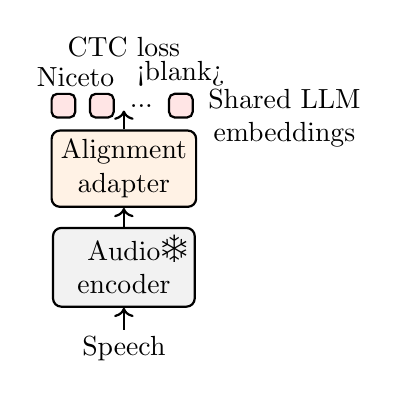
\begin{tikzpicture} [scale=0.8]
        \node(ae) at (0,0) [rectangle, draw=black, fill=gray!10, rounded corners=3pt, thick, minimum width=1.8cm,minimum height=1cm,align=center] {Audio\\encoder};
        \node(freeze) at ([xshift=0.8cm,yshift=0.3cm]ae.center) [rectangle, align=center] {\Large{\ding{100}}};
        \node(fb) at ([yshift=-0.3cm]ae.south) [rectangle, align=center,anchor=north] {Speech};
        \node(aa) at ([yshift=0.3cm]ae.north) [rectangle, draw=black, fill=orange!10, rounded corners=3pt, thick, minimum width=1.8cm,minimum height=0.5cm,align=center,anchor=south] {Alignment\\adapter};
        
        \node(f1) at ([yshift=1.0cm]aa.west) [rectangle, draw=black, fill=red!10, rounded corners=2pt, thick, minimum width=0.3cm, minimum height=0.3cm,align=center,anchor=west] {};
        \node(f2) at ([xshift=0.2cm]f1.east) [rectangle, draw=black, fill=red!10, rounded corners=2pt, thick, minimum width=0.3cm, minimum height=0.3cm,align=center,anchor=west] {};
        \node(f3) at ([xshift=0.075cm]f2.east) [rectangle, draw=white,  thick, align=center,anchor=west] {...};
        \node(f4) at ([xshift=0.075cm]f3.east) [rectangle, draw=black, fill=red!10, rounded corners=2pt, thick, minimum width=0.3cm, minimum height=0.3cm,align=center,anchor=west] {};
        \node(t1) at ([yshift=-0.05cm]f1.north) [rectangle, align=center,anchor=south] {Nice};
        \node(t2) at ([yshift=-0.05cm]f2.north) [rectangle, align=center,anchor=south] {to};
        \node(t4) at ([yshift=-0.05cm]f4.north) [rectangle, align=center,anchor=south] {<blank>};
        \node(se) at ([xshift=0.075cm,yshift=-0.2cm]f4.east) [rectangle, align=center,anchor=west] {Shared LLM\\embeddings};
        \node(ctc) at ([yshift=1.0cm]aa.north) [rectangle, rounded corners=3pt, thick, align=center,anchor=south] {CTC loss};

        
        \draw[->,thick]([yshift=-0.05cm]fb.north)--(ae.south);
        \draw[->,thick](ae.north)--(aa.south);
        \draw[->,thick](aa.north)--([yshift=0.3cm]aa.north);

        
      \end{tikzpicture}
    \end{minipage}
    }
    \subfigure[Shrinking stage]{
    \begin{minipage}[t]{0.45\linewidth}
    \centering
    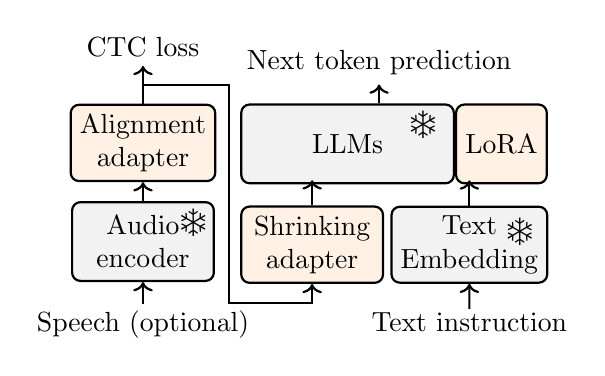
\begin{tikzpicture} [scale=0.8]
        \node(ae) at (0,0) [rectangle, draw=black, fill=gray!10, rounded corners=3pt, thick, minimum width=1.8cm,minimum height=1cm,align=center] {Audio\\encoder};
        \node(freeze) at ([xshift=0.8cm,yshift=0.3cm]ae.center) [rectangle, align=center] {\Large{\ding{100}}};
        \node(fb) at ([yshift=-0.3cm]ae.south) [rectangle, align=center,anchor=north] {Speech (optional)};
        \node(aa) at ([yshift=0.3cm]ae.north) [rectangle, draw=black, fill=orange!10, rounded corners=3pt, thick, minimum width=1.8cm,minimum height=0.5cm,align=center,anchor=south] {Alignment\\adapter};
        \node(ctc) at ([yshift=0.6cm]aa.north) [rectangle,align=center,anchor=south] {CTC loss};
        \node(sa) at ([xshift=0.4cm,yshift=-0.05cm]ae.east) [rectangle, draw=black, fill=orange!10, rounded corners=3pt, thick, minimum width=1.8cm,minimum height=0.5cm,align=center,anchor=west] {Shrinking\\adapter};
        \node(llm) at ([yshift=1.6cm]sa.west) [rectangle, draw=black, fill=gray!10, rounded corners=3pt, thick, minimum width=2.7cm,minimum height=1.0cm,align=center,anchor=west] {LLMs};
        \node(lora) at (llm.east) [rectangle, draw=black, fill=orange!10, rounded corners=3pt, thick, minimum width=1.0cm,minimum height=1.0cm,align=center,anchor=west] {LoRA};
        \node(te) at ([xshift=0.1cm]sa.east) [rectangle, draw=black, fill=gray!10, rounded corners=3pt, thick, minimum width=1.8cm,minimum height=0.5cm,align=center,anchor=west] {Text\\Embedding};
        \node(freeze3) at ([xshift=0.8cm,yshift=0.2cm]te.center) [rectangle, align=center] {\Large{\ding{100}}};
        \node(ti) at ([yshift=-0.3cm]te.south) [rectangle, align=center,anchor=north] {Text instruction};
        \node(freeze2) at ([xshift=1.2cm,yshift=0.3cm]llm.center) [rectangle, align=center] {\Large{\ding{100}}};
        \node(loss) at ([xshift=0.5cm, yshift=0.3cm]llm.north) [rectangle, align=center,anchor=south] {Next token prediction};

        
        \draw[->,thick]([yshift=-0.05cm]fb.north)--(ae.south);
        \draw[->,thick](ae.north)--(aa.south);
        \draw[->,thick](aa.north)--(ctc.south);
        \draw[->,thick](sa.north)--([yshift=0.4cm]sa.north);
        \draw[->,thick](te.north)--([yshift=0.4cm]te.north);
        \draw[->,thick]([yshift=-0.3cm]loss.south)--(loss.south);
        \draw[->,thick]([yshift=-0.1cm]ti.north)--(te.south);

        \draw[->,thick](aa.north)--([yshift=0.3cm]aa.north)--([xshift=0.2cm, yshift=0.3cm]aa.north -| aa.east)--([xshift=0.2cm, yshift=-0.3cm]sa.south -| aa.east)--([yshift=-0.3cm]sa.south)--(sa.south);
      \end{tikzpicture}
    \end{minipage}
    }
    \subfigure[SFT stage]{
    \begin{minipage}[t]{0.20\linewidth}
    \centering
    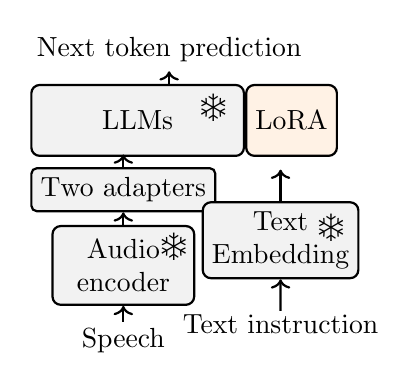
\begin{tikzpicture} [scale=0.8]
        \node(ae) at (0,0) [rectangle, draw=black, fill=gray!10, rounded corners=3pt, thick, minimum width=1.8cm,minimum height=1cm,align=center] {Audio\\encoder};
        \node(freeze) at ([xshift=0.8cm,yshift=0.3cm]ae.center) [rectangle, align=center] {\Large{\ding{100}}};
        \node(fb) at ([yshift=-0.2cm]ae.south) [rectangle, align=center,anchor=north] {Speech};
        \node(aa) at ([yshift=0.2cm]ae.north) [rectangle, draw=black, fill=gray!10, rounded corners=2pt, thick, minimum width=1.8cm,minimum height=0.5cm,align=center,anchor=south] {Two adapters};
        
        \node(llm) at ([yshift=1.1cm]aa.west) [rectangle, draw=black, fill=gray!10, rounded corners=3pt, thick, minimum width=2.7cm,minimum height=0.9cm,align=center,anchor=west] {LLMs};
        \node(lora) at (llm.east) [rectangle, draw=black, fill=orange!10, rounded corners=3pt, thick, minimum width=0.9cm,minimum height=0.9cm,align=center,anchor=west] {LoRA};
        \node(te) at ([xshift=0.1cm,yshift=0.4cm]ae.east) [rectangle, draw=black, fill=gray!10, rounded corners=3pt, thick, minimum width=1.8cm,minimum height=0.5cm,align=center,anchor=west] {Text\\Embedding};
        \node(freeze3) at ([xshift=0.8cm,yshift=0.2cm]te.center) [rectangle, align=center] {\Large{\ding{100}}};
        \node(ti) at ([yshift=-0.4cm]te.south) [rectangle, align=center,anchor=north] {Text instruction};
        \node(freeze2) at ([xshift=1.2cm,yshift=0.2cm]llm.center) [rectangle, align=center] {\Large{\ding{100}}};
        \node(loss) at ([xshift=0.5cm, yshift=0.2cm]llm.north) [rectangle, align=center,anchor=south] {Next token prediction};
       
        \draw[->,thick]([yshift=-0.05cm]fb.north)--(ae.south);
        \draw[->,thick](ae.north)--(aa.south);
        \draw[->,thick](aa.north)--([yshift=0.2cm]aa.north);
        \draw[->,thick](te.north)--([yshift=0.5cm]te.north);
        \draw[->,thick]([yshift=-0.2cm]loss.south)--(loss.south);
        \draw[->,thick]([yshift=-0.1cm]ti.north)--(te.south);
        
      \end{tikzpicture}
    \end{minipage}
    }
      \caption{Training progress of Soundwave. The gray modules are frozen while the orange modules are updated.}
      \label{architecture}
  \end{figure*}

  

\paragraph{Model Architecture.}

The architecture of $f_{\theta_{W_i}}\left(u_i, \delta_{i+1}\right)$, named \method{}, is shown in Figure~\ref{fig:arch} and defined as follows:
\begin{align}
    \left[\bar{u}_i, \bar{\delta}_{i+1}\right]&=\mathrm{Norm}\left(\left[u_i, \delta_{i+1}\right]\right)\\
    h_i&=\theta_2\mathrm{Dropout}\left(\theta_1\left[\bar{u}_i, \bar{\delta}_{i+1}\right]\right)\\
    \left[\tilde{u}_i, \tilde{\delta}_{i+1}\right]&=h_i + \left[\bar{u}_i, \bar{\delta}_{i+1}\right]
\end{align}
where $\theta_1 \in \mathbb{R}^{r \times 2d}$ and $\theta_2 \in \mathbb{R}^{2d \times r}$ are the optimizer parameters with $r \ll d$. $[\cdot]$ denotes the vector concatenation. $\mathrm{Norm}$ normalizes $u_i$ and $\delta_{i+1}$ to have zero mean and unit variance separately. $\mathrm{Dropout}$ is the dropout regularization~\cite{DBLP:journals/jmlr/SrivastavaHKSS14}. In practice, $\theta_1$ and $\theta_2$ are shared across all weights with the same shape. \method{} is similar to the Bottleneck Adapter~\cite{DBLP:conf/icml/HoulsbyGJMLGAG19}, with the key difference that its input is gradients and its output is the weight update. As such, \method{} can also be regarded as a specialized PEFT technique tailored to reasoning.

% \textcolor{red}{a two-column workflow diagram}

\begin{table*}
\centering
% \footnotesize
\resizebox{\linewidth}{!}{
% \setlength{\tabcolsep}{5pt}
\begin{tabular}[t]{l|llll|c}
\toprule
 \makecell[c]{\textbf{Method}} & \makecell[c]{\textbf{MATH}} & \makecell[c]{\textbf{GSM8K}} & \makecell[c]{\textbf{MBPP}} & \makecell[c]{\textbf{HumanEval}} & \makecell[c]{\textbf{Avg.}} \\
\midrule
\multicolumn{6}{c}{\texttt{Llama-3.1-8B-Instruct}} \\
\midrule
Revision~\cite{DBLP:journals/corr/abs-2408-03314} & 0.2960 & 0.4570 & 0.2991 & 0.3889 & 0.3603 \\
Beam Search~\cite{ow1988filtered} & 0.2560 & 0.4842 & 0.1869 & 0.2407 & 0.2920 \\
% Beam Search Sampling~\cite{DBLP:journals/corr/abs-1910-03771} & 0.2520$_{0.0000}$ & 0.4842$_{0.0000}$ & 0.1822$_{0.0000}$ & 0.2407$_{0.0000}$ & 0.2898 \\
Self-Consistency~\cite{DBLP:conf/iclr/0002WSLCNCZ23} & 0.3000$_{0.0057}$ & 0.4525$_{0.0111}$ & 0.1371$_{0.0180}$ & 0.1235$_{0.0531}$ & 0.2533 \\
Self-Refine~\cite{DBLP:conf/nips/MadaanTGHGW0DPY23} & 0.4693$_{0.0207}$ & 0.7828$_{0.0064}$ & 0.2305$_{0.0088}$ & 0.2963$_{0.0800}$ & 0.4447 \\
Best-of-N~\cite{DBLP:journals/corr/abs-2407-21787} & 0.6427$_{0.0154}$ & \underline{0.8069}$_{0.0043}$ & \underline{0.5452}$_{0.0154}$ & 0.6728$_{0.0087}$ & 0.6669 \\
\midrule
FTTT & \underline{0.6707}$_{0.0222}$ & \textbf{0.8100}$_{0.0037}$ & \textbf{0.5607}$_{0.0212}$ & \textbf{0.6852}$_{0.0302}$ & 0.6817 \\
+ w/o Self-Reflected Feedback & \textbf{0.6720}$_{0.0113}$ & 0.8054$_{0.0133}$ & 0.5405$_{0.0117}$ & \underline{0.6790}$_{0.0087}$ & 0.6742 \\
\toprule
\multicolumn{6}{c}{\texttt{Mistral-7B-Instruct-v0.3}} \\
\midrule
Revision~\cite{DBLP:journals/corr/abs-2408-03314} & 0.0497 & 0.1686 & 0.1351 & 0.1000 & 0.1134 \\
Beam Search~\cite{ow1988filtered} & 0.1783 & 0.4537 & 0.1318 & 0.1600 & 0.2310 \\
% Beam Search Sampling~\cite{DBLP:journals/corr/abs-1910-03771} & 0.1716$_{0.0032}$ & 0.4533$_{0.0016}$ & 0.1318$_{0.0000}$ & 0.1500$_{0.0000}$ & 0.2267 \\
Self-Consistency~\cite{DBLP:conf/iclr/0002WSLCNCZ23} & 0.1618$_{0.0011}$ & 0.3549$_{0.0052}$ & 0.1243$_{0.0135}$ & 0.1033$_{0.0236}$ & 0.1861 \\
Self-Refine~\cite{DBLP:conf/nips/MadaanTGHGW0DPY23} & 0.1287$_{0.0139}$ & 0.3312$_{0.0078}$ & 0.2347$_{0.0091}$ & 0.3533$_{0.0309}$ & 0.2620 \\
Best-of-N~\cite{DBLP:journals/corr/abs-2407-21787} & 0.4688$_{0.0138}$ & 0.7807$_{0.0055}$ & \textbf{0.4962}$_{0.0171}$ & 0.6500$_{0.0141}$ & 0.5989 \\
\midrule
FTTT & \underline{0.4733}$_{0.0087}$ & \underline{0.7820}$_{0.0045}$ & \textbf{0.4962}$_{0.0015}$ & \underline{0.6633}$_{0.0125}$ & 0.6037 \\
+ w/o Self-Reflected Feedback & \textbf{0.4876}$_{0.0133}$ & \textbf{0.7858}$_{0.0021}$ & \underline{0.4941}$_{0.0040}$ & \textbf{0.6833}$_{0.0205}$ & 0.6127 \\
\bottomrule
\end{tabular}
}
% \vspace{-5pt}
\caption{Experimental results on four datasets with a budget of 32. For stochastic algorithms, we report the mean of three runs with different random seeds and standard deviation in the subscript. \textbf{Bold} entries are the best results, and \underline{underlined} entries are the second-best results.}
\label{tab:pilot}
% \vspace{-0.5cm}
\end{table*}

\section{Experiments}
\label{sec:exp}

\subsection{Setup}

\paragraph{Datasets.}

We evaluate both baselines and our method on math and coding reasoning tasks:
(a) Mathematical reasoning: MATH~\cite{DBLP:conf/nips/HendrycksBKABTS21} and GSM8K~\cite{DBLP:journals/corr/abs-2110-14168}, using the test split from~\citet{DBLP:conf/iclr/LightmanKBEBLLS24} for MATH.
(b) Code generation: MBPP~\cite{DBLP:journals/corr/abs-2108-07732} and HumanEval~\cite{DBLP:journals/corr/abs-2107-03374}.
For all datasets, we report results on subsets where models fail with greedy decoding. We use Exact Match as the evaluation metric as well as the verifier for math tasks and Pass@1 for code.

\paragraph{Models.}

We conduct experiments with \texttt{Llama-3.1-8B-Instruct}~\cite{DBLP:journals/corr/abs-2407-21783} and \texttt{Mistral-7B-Instruct-v0.3}~\cite{DBLP:journals/corr/abs-2310-06825}.
We evaluate both models with zero-shot prompting and follow the official instructions when evaluating the model on each dataset\footnote{\url{https://huggingface.co/datasets/meta-llama/Llama-3.1-8B-Instruct-evals}}.

\paragraph{Baselines.}

We compare FTTT with the following test-time scaling methods:
\begin{itemize}[noitemsep, nolistsep]
    \item \textbf{Beam Search}~\cite{ow1988filtered} is a popular search algorithm that approximates the most confident model prediction.
    % \item \textbf{Self-Evaluation Guided Beam Search}~\cite{DBLP:conf/nips/XieKZZKHX23}
    % \item \textbf{Stochastic Beam Search}~\cite{DBLP:conf/icml/KoolHW19}
    % \item \textbf{Beam Search Sampling}~\cite{DBLP:journals/corr/abs-1910-03771} is a randomized version of beam search. Instead of keeping the top-$B$ candidates deterministically, it samples them stochastically to avoid similar predictions, where $B$ is the beam size. The best prediction is finally selected based on feedback.
    \item \textbf{Self-Consistency}~\cite{DBLP:conf/iclr/0002WSLCNCZ23} samples multiple predictions and selects the most frequent answer.
    \item \textbf{Best-of-N}~\cite{DBLP:journals/corr/abs-2407-21787} samples $N$ predictions independently and picks the best one based on external feedback.
    \item \textbf{Revision}~\cite{DBLP:journals/corr/abs-2408-03314} iteratively refines answers by conditioning the model on previous attempts.
    \item \textbf{Self-Refine}~\cite{DBLP:conf/nips/MadaanTGHGW0DPY23} alternates between self-critique and refinement. We select the best solution based on feedback.
\end{itemize}

\begin{figure}[t] % 1-column
\footnotesize
\centering 

% Adjust the image width to fit within one column
\newcommand{\imgwidth}{0.18\linewidth} % Set image width to 16% of the line width

% 1st Image
\begin{tikzpicture}[x=1cm, y=1cm]
    \node[anchor=south] (FigA1) at (0,0) {
        \includegraphics[width=\imgwidth]{Fig./Qual/imgs/ip2p_sub/shark/src_img.jpg}
    };
    \node[anchor=south, yshift=-1.5mm] at (FigA1.north) {\footnotesize Source};
\end{tikzpicture}\hspace{-1mm}%
% 2nd Image
\begin{tikzpicture}[x=1cm, y=1cm]
    \node[anchor=south] (FigB1) at (0,0) {
        \includegraphics[width=\imgwidth]{Fig./Qual/imgs/ip2p_sub/shark/dds.jpg}
    };
    \node[anchor=south, yshift=-1.5mm] at (FigB1.north) {\footnotesize DDS};
\end{tikzpicture}\hspace{-1mm}%
\begin{tikzpicture}[x=1cm, y=1cm]
    \node[anchor=south] (FigB1) at (0,0) {
        \includegraphics[width=\imgwidth]{Fig./Qual/imgs/ablation/scale/scale_0.4-iter_1-optimstep_200.jpg}
    };
    \node[anchor=south, yshift=-1.5mm] at (FigB1.north) {\footnotesize $\lambda=0.4$};
\end{tikzpicture}\hspace{-1mm}%
% % 3rd Image
\begin{tikzpicture}[x=1cm, y=1cm]
    \node[anchor=south] (FigC1) at (0,0) {
        \includegraphics[width=\imgwidth]{Fig./Qual/imgs/ablation/scale/scale_0.8-iter_1-optimstep_200.jpg}
    };
    \node[anchor=south, yshift=-1.5mm] at (FigC1.north) {\footnotesize $\lambda=0.8$};
\end{tikzpicture}\hspace{-1mm}%
% 4th Image
\begin{tikzpicture}[x=1cm, y=1cm]
    \node[anchor=south] (FigD1) at (0,0) {
        \includegraphics[width=\imgwidth]{Fig./Qual/imgs/ablation/scale/scale_1.0-iter_1-optimstep_200.jpg}
    };
    \node[anchor=south, yshift=-1.5mm] at (FigD1.north) {\footnotesize $\lambda=1.0$};
\end{tikzpicture}
\vspace{-3pt}
% Caption Text
\setulcolor{magenta}
\setul{0.3pt}{2pt}
\centering \textit{``A photo of shark" $\to$ ``A photo of \ul{dolphin}"} 
\vspace{-6pt}
\caption{\textbf{Ablation study} on scale $\lambda$. To show the effect of scale more extremely, the number of iterations of FPR is set as 1. The result of DDS is the same as $\lambda=0$ since it means no update for source identity.}
\vspace{-10pt}
\label{fig:ablation_scale}
\end{figure}


For sampling-based methods, we use nucleus sampling~\cite{DBLP:conf/iclr/HoltzmanBDFC20} with a temperature of 0.6 and $p=0.95$, following~\citet{DBLP:journals/corr/abs-2407-21787}. All methods are allocated a budget of 32. For FTTT, we fine-tune the model with LoRA~\cite{DBLP:conf/iclr/HuSWALWWC22}, using a rank of 4 and a dropout ratio of 0.05. We use the Adam optimizer~\cite{DBLP:journals/corr/KingmaB14} with a learning rate of 1e-5, except for \texttt{Mistral-7B-Instruct-v0.3} in coding tasks, where we use 2e-5.

As \method{} is a specialized PEFT method, we compare it with the following PEFT approaches: \textbf{Adapter}~\cite{DBLP:conf/icml/HoulsbyGJMLGAG19}, \textbf{(IA)$^3$}~\cite{DBLP:conf/nips/LiuTMMHBR22}, \textbf{LoRA}~\cite{DBLP:conf/iclr/HuSWALWWC22} and \textbf{LN-Tuning}~\cite{DBLP:conf/iclr/ZhaoT0MX24}. We also include \textbf{full fine-tuning} that updates all LLM weights. For \method{}, $r=16$ and the dropout ratio is 0.1. We only apply \method{} to the query and value projections in the last two layers of the LLM. Detailed configurations are in Appendix~\ref{app:setting}.

% BitFit~\cite{ben-zaken-etal-2022-bitfit}

% ReFT~\cite{DBLP:journals/corr/abs-2404-03592}

% \textbf{Prefix-Tuning}~\cite{li-liang-2021-prefix}

\subsection{Training-Free Results}
\label{sec:result1}

Table~\ref{tab:pilot} compares FTTT with various baselines across four reasoning datasets. FTTT, both with and without self-reflected feedback, outperforms conventional test-time scaling methods on average. This success is partially explained by the findings of \citet{ye2024physicslanguagemodels22}, which show that training with error-correction data enhances reasoning capabilities and models do not retry during inference. FTTT is also efficient. For instance, the inference time of \texttt{Llama-3.1-8B-Instruct} on GSM8K with a budget of 32 is 3 GPU hours for the best parallel sampling method (Best-of-N) and 20 GPU hours for the best sequential revision method (Self-Refine). In contrast, FTTT achieves inference times of approximately 3 GPU hours without self-reflected feedback and 4 GPU hours with self-reflected feedback.

% the inference time of \texttt{Llama-3.1-8B-Instruct} with FTTT on GSM8K is 46 minutes on 4 NVIDIA H800, while for Best-of-N and Self-Refine, their inference time is 47 minutes and 5 hours

Notably, self-reflected feedback does not always improve results. Its effectiveness appears to depend on the LLM's self-reflection ability. To test this, we computed the Spearman rank correlation between FTTT and Self-Refine, a self-reflection-based algorithm. The Spearman coefficient ($r = 0.8656$, $p \leq 0.05$) indicates a strong positive correlation, supporting our hypothesis. We also observe that Self-Consistency performs poorly on code tasks because sampled code snippets rarely match exactly, making majority voting akin to random selection.

Figure~\ref{fig:scale} illustrates performance for FTTT and baselines under varying budgets. FTTT consistently outperforms baselines, with greater gains under constrained budgets. In contrast, Revision and Self-Consistency do not scale well. Revision struggles with long-context reasoning due to length generalization issues~\cite{li-etal-2024-making}, while Self-Consistency fails to leverage feedback, often discarding correct answers during majority voting due to long-tailed distributions of correct answers~\cite{DBLP:journals/corr/abs-2407-21787}.

% a line plot that shows the number of additional problems solved given more budgets

% the portion of problems solved in different difficulty levels in MATH

\subsection{Fine-Tuning Results}

%% complete the rights form.
\copyrightyear{2025}
\acmYear{2025}
\setcopyright{cc}
\setcctype{by}
\acmConference[WWW '25]{Proceedings of the ACM Web Conference 2025}{April 28-May 2, 2025}{Sydney, NSW, Australia}
\acmBooktitle{Proceedings of the ACM Web Conference 2025 (WWW '25), April 28-May 2, 2025, Sydney, NSW, Australia}
\acmDOI{10.1145/3696410.3714923}
\acmISBN{979-8-4007-1274-6/25/04}
%%
%%  Uncomment \acmBooktitle if the title of the proceedings is different
%%  from ``Proceedings of ...''!
%%
%%\acmBooktitle{Woodstock '18: ACM Symposium on Neural Gaze Detection,
%%  June 03--05, 2018, Woodstock, NY}

%%
%% The code below is generated by the tool at http://dl.acm.org/ccs.cfm.
%% Please copy and paste the code instead of the example below.
%%

%%
%% Keywords. The author(s) should pick words that accurately describe
%% the work being presented. Separate the keywords with commas.
% \keywords{Beyond-accuracy metrics}
\begin{CCSXML}
<ccs2012>
   <concept>
       <concept_id>10010147.10010178.10010179.10003352</concept_id>
       <concept_desc>Computing methodologies~Information extraction</concept_desc>
       <concept_significance>500</concept_significance>
       </concept>
   <concept>
       <concept_id>10010147.10010178.10010219.10010220</concept_id>
       <concept_desc>Computing methodologies~Multi-agent systems</concept_desc>
       <concept_significance>500</concept_significance>
       </concept>
 </ccs2012>
\end{CCSXML}

\ccsdesc[500]{Computing methodologies~Information extraction}
\ccsdesc[500]{Computing methodologies~Multi-agent systems}

\keywords{Information extraction, Named entity recognition, Zero-shot learning, Large language models, Multi-agent systems}
%% A "teaser" image appears between the author and affiliation
%% information and the body of the document, and typically spans the
%% page.
% -

%\received{20 February 2007}
%\received[revised]{12 March 2009}
%\received[accepted]{5 June 2009}

%%
%% This command processes the author and affiliation and title
%% information and builds the first part of the formatted document.

\begin{table}[t]
\caption{Experimental results of fine-tuning baselines on RefDrone benchmark. Top groups: specialist models. Bottom groups: LMMs for REC tasks.}

\label{tab:finetune}
  \centering
\begin{adjustbox}{width=\linewidth}
  \begin{tabular}{l c  c c c }
    \toprule
    Methods & F1$_{inst.}$ & Acc$_{inst.}$ & F1$_{img.}$ & Acc$_{img.}$ \\
    \midrule 

MDETR~\cite{mdetr}  & 32.60 & 19.49 & 19.17 & 10.81 \\
GLIP~\cite{glip} & 24.23 & 14.86 & 16.92 & 13.29  \\
GDINO-T~\cite{gdino}  & 30.50 & 19.02 & 29.65 & 21.07 \\
NGDINO-T (Ours) &  33.34 & 20.98  & 32.45  & 22.84 \\
GDINO-B~\cite{gdino}  & 31.96 & 19.99 & 31.69 & 22.26 \\
NGDINO-B (Ours)&  \textbf{34.44} &\textbf{ 21.76 } & \textbf{34.01}  & \textbf{23.89 }\\

\midrule

MiniGPT-v2~\cite{chen2023minigpt}  & 4.97 & 2.74 & 13.56 & 8.97 \\
LLaVA~\cite{llava} & 6.00 & 3.63 & 14.43 & 11.57 \\
Qwen-VL~\cite{bai2023qwen} &  14.14 & 7.61 & 20.10 & 11.17 \\
RDAgent (Ours) & \textbf{ 58.14} & \textbf{41.13}  &\textbf{ 37.07}  & \textbf{23.54 }\\


  \bottomrule

\end{tabular}
\end{adjustbox}

\end{table}

We present the results of PEFT baselines and \method{} with a budget of 32 in Table~\ref{tab:meta}. Best-of-N is applied to PEFT baselines to exploit test-time feedback. HumanEval is excluded as it lacks a training set. Table~\ref{tab:meta} highlights the effectiveness of \method{}, outperforming all PEFT baselines by at least 2.58\% on average. \method{} is also parameter-efficient, with 439K trainable parameters that are comparable to the most lightweight PEFT method (LN-Tuning, 266K parameters), while surpassing the best PEFT method (LoRA, 1.7M parameters) with an order of magnitude fewer parameters.
However, \method{} shows suboptimal performance on MATH for \texttt{Mistral-7B-Instruct-v0.3}, which is consistent with other PEFT methods with few trainable parameters (e.g., (IA)$^3$, LoRA, LN-Tuning). This is likely due to \texttt{Mistral-7B-Instruct-v0.3}'s limited mathematical reasoning capabilities, requiring significant parameter updates to improve performance in this domain.

\method{} incurs negligible inference overhead. For example, on GSM8K with \texttt{Llama-3.1-8B-Instruct} and a budget of 32, the best test-time scaling baseline (FTTT) requires 4 GPU hours, whereas \method{} uses only 1.5 GPU hours, benefiting from shorter yet accurate predictions.

% fastest adapter 6.5 GPU hours

% !TEX root = main.tex

\begin{figure}[t]
\vspace{-1.5cm}
\begin{minipage}{0.34\textwidth}
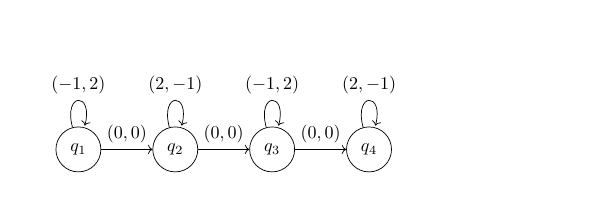
\begin{tikzpicture}[scale=0.25]
\usetikzlibrary{automata, positioning}
\scalebox{0.65}{
\node[state] (q1) {$q_1$};
\node[state, right=of q1] (q2) {$q_2$};
\node[state, right=of q2] (q3) {$q_3$};
\node[state, right=of q3] (q4) {$q_4$};

\path[->] (q1) edge [loop above] node[above] {$(-1,2)$} (q1) edge node[above] {$(0,0)$} (q2); 
\path[->] (q2) edge [loop above] node[above] {$(2,-1)$} (q2) edge node[above] {$(0,0)$} (q3);
\path[->] (q3) edge [loop above] node[above] {$(-1,2)$} (q3) edge node[above] {$(0,0)$} (q4);
\path[->] (q4) edge [loop above] node[above] {$(2,-1)$} (q4);
}
\end{tikzpicture}
\end{minipage}
\begin{minipage}{0.32\textwidth}
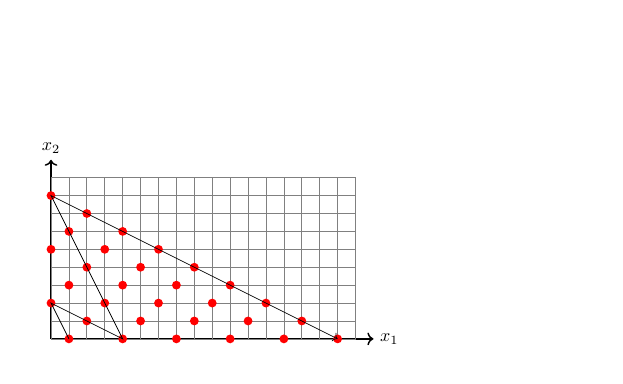
\begin{tikzpicture}[scale=0.35]
\scalebox{0.65}{
\draw[->, thick] (0, 0) -- (18, 0) node[right] {$x_1$};
\draw[->, thick] (0, 0) -- (0, 10) node[above] {$x_2$};

\draw[step=1, gray, thin] (0, 0) grid (17, 9);

\foreach \x in {1,4,7,10,13,16} \fill[red] (\x,0) circle (7pt);
\foreach \x in {2,5,8,11,14} \fill[red] (\x,1) circle (7pt);
\foreach \x in {0,3,6,9,12} \fill[red] (\x,2) circle (7pt);
\foreach \x in {1,4,7,10} \fill[red] (\x,3) circle (7pt);
\foreach \x in {2,5,8} \fill[red] (\x,4) circle (7pt);
\foreach \x in {0,3,6} \fill[red] (\x,5) circle (7pt);
\foreach \x in {1,4} \fill[red] (\x,6) circle (7pt);
\foreach \x in {2} \fill[red] (\x,7) circle (7pt);
\foreach \x in {0} \fill[red] (\x,8) circle (7pt);

\draw[->] (1,0) -- (0,2) -- (2,1) -- (4,0) -- (3,2) -- (2,4) -- (1,6) -- (0,8) -- (2,7) -- (4,6) -- (6,5) -- (8,4) -- (10,3) -- (12,2) -- (14,1) -- (16,0);
}
\end{tikzpicture}
\end{minipage}
\begin{minipage}{0.32\textwidth}
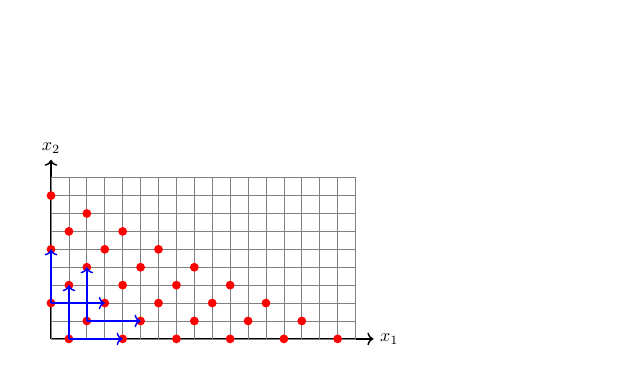
\begin{tikzpicture}[scale=0.35]
\scalebox{0.65}{
\draw[->, thick] (0, 0) -- (18, 0) node[right] {$x_1$};
\draw[->, thick] (0, 0) -- (0, 10) node[above] {$x_2$};

\draw[step=1, gray, thin] (0, 0) grid (17, 9);

\foreach \x in {1,4,7,10,13,16} \fill[red] (\x,0) circle (7pt);
\foreach \x in {2,5,8,11,14} \fill[red] (\x,1) circle (7pt);
\foreach \x in {0,3,6,9,12} \fill[red] (\x,2) circle (7pt);
\foreach \x in {1,4,7,10} \fill[red] (\x,3) circle (7pt);
\foreach \x in {2,5,8} \fill[red] (\x,4) circle (7pt);
\foreach \x in {0,3,6} \fill[red] (\x,5) circle (7pt);
\foreach \x in {1,4} \fill[red] (\x,6) circle (7pt);
\foreach \x in {2} \fill[red] (\x,7) circle (7pt);
\foreach \x in {0} \fill[red] (\x,8) circle (7pt);

\draw[->,blue,thick] (1,0) -- (4,0);
\draw[->,blue,thick] (1,0) -- (1,3);

\draw[->,blue,thick] (2,1) -- (5,1);
\draw[->,blue,thick] (2,1) -- (2,4);

\draw[->,blue,thick] (0,2) -- (3,2);
\draw[->,blue,thick] (0,2) -- (0,5);
}
\end{tikzpicture}
\end{minipage}
\caption{Left: 4-component \dvass $V_2$. 
Middle: the set $\reach_{q_4}(V_2, q_1(1,0))$ and a path $q_1(1,0) \tran q_4(16,0)$.
Right: bases 
%$A = \{(1,0),(2,1),(0,2)\}$ 
and periods 
%$P = \{(0,3),(3,0)\}$
 of an over-approximating semi-linear set $A+P^*$.}
\label{fig:zigzag}
\end{figure}

\begin{example}
For $k\geq 1$, let $V_k$ be a $(2k)$-component \dvass, where each component has just one state $q_i$
and one transition:
$(q_i, (-1,2), q_i)$ for odd $i$, and $(q_i, (2,-1), q_i)$ for even $i$.
Bridge transitions are $(q_i, (0,0), q_{i+1})$.
Figure~\ref{fig:zigzag} shows $V_2$ (left) and 
a path in $V_2$ from $s = q_1(1,0)$ to $t = q_4(16,0)$ together with 
the reachability set $\reach_{q_4}(V_2, s)$ (middle).
In general,
\begin{align} \label{eq:reachk}
X_k := \reach_{q_{2k}}(V_k, s) \ = \ \set{(x_1,x_2) \mid x_1+2x_2 \leq 4^k, \  x_1+2x_2 \equiv 1 \!\! \mod 3}.
\end{align}
Even if the size of the reachability set is 
exponential in $k$, for small $(x_1, x_2)$ it is periodic and the periods are small.
The set $X_k$ can be over-approximated by $A + P^*$ for $A = \set{(1,0),(2,1),(0,2)}$ and $P = \set{(0,3),(3,0)}$
(shown on the right of Figure~\ref{fig:zigzag}), namely for every $k\geq 1$ and $B\in\N$,
the set $X_k$ is \kanapka {$8$} {$B$}. 
For illustration, consider $Y := X_k \cap ((1,0) + P^*)$.
If $(1,0) + P^{\leq B} \subseteq X_k$ then $Y$ is a $B$-approximation
of $(1,0) + P^*$ with $\norm((1,0)), \norm(P) \leq 3 \leq 8$. 
Otherwise, there is some $(v_1, v_2) \in \big((1,0) + P^{\leq B}\big)\setminus X_k$, and
then $B$ is larger than $4^k$:
\[
%8B \geq 2(1 + 3B) \geq 2(v_1 + v_2) \geq v_1 + 2 v_2 > 
4^k < v_1 + 2 v_2 \leq 2(v_1 + v_2) \leq 2(1+3B) \leq 8B.
\]
Therefore by \eqref{eq:reachk}, each $(x_1,x_2) \in Y$ satisfies 
$\norm(x_1,x_2) = x_1 + x_2 \leq x_1 + 2x_2 \leq 4^k < 8B$, and thus
$Y$, seen as a union of singletons, is a union of 
linear sets with norm of base bounded by $8B$ and empty set of periods. 
In both cases, 
$Y$ is \kanapka {$8$} {$B$}. 
%The same intuition stays behind polynomial approximability of \dvass stated in Lemma~\ref{lem:2vass-sandwich}.
\end{example}

Finally, Figure~\ref{fig:tune-scale} examines the scaling behavior of PEFT baselines and \method{}. Initially, \method{} underperforms compared to other PEFT methods and FTTT, but it mostly achieves superior results when the budget exceeds 2. \method{}'s weaker performance with smaller budgets arises from its reliance on an initial attempt sampled from the raw LLM to initiate the process. This initial attempt often fails but is still counted as a valid attempt, making \method{} less competitive in low-budget settings.

\subsection{Analysis}

\paragraph{Ablation Study.}

Table~\ref{tab:ablation} presents an ablation study on the architecture design of \method{}. The results demonstrate that all components are essential, as removing any of them significantly degrades performance. Notably, normalization is the most critical component, as it addresses the varying gradient scales of different weights.

% how to combine predicted updates when scaling

\paragraph{Case Study.}

Table~\ref{tab:case} provides two examples on GSM8K where the leading PEFT method, LoRA, fails, but \method{} succeeds using \texttt{Llama-3.1-8B-Instruct}. These examples highlight \method{}'s superior ability to correctly interpret and reason through questions, unlike LoRA.

% \begin{table}[!t]
% \centering
% \scalebox{0.68}{
%     \begin{tabular}{ll cccc}
%       \toprule
%       & \multicolumn{4}{c}{\textbf{Intellipro Dataset}}\\
%       & \multicolumn{2}{c}{Rank Resume} & \multicolumn{2}{c}{Rank Job} \\
%       \cmidrule(lr){2-3} \cmidrule(lr){4-5} 
%       \textbf{Method}
%       &  Recall@100 & nDCG@100 & Recall@10 & nDCG@10 \\
%       \midrule
%       \confitold{}
%       & 71.28 &34.79 &76.50 &52.57 
%       \\
%       \cmidrule{2-5}
%       \confitsimple{}
%     & 82.53 &48.17
%        & 85.58 &64.91
     
%        \\
%        +\RunnerUpMiningShort{}
%     &85.43 &50.99 &91.38 &71.34 
%       \\
%       +\HyReShort
%         &- & -
%        &-&-\\
       
%       \bottomrule

%     \end{tabular}
%   }
% \caption{Ablation studies using Jina-v2-base as the encoder. ``\confitsimple{}'' refers using a simplified encoder architecture. \framework{} trains \confitsimple{} with \RunnerUpMiningShort{} and \HyReShort{}.}
% \label{tbl:ablation}
% \end{table}
\begin{table*}[!t]
\centering
\scalebox{0.75}{
    \begin{tabular}{l cccc cccc}
      \toprule
      & \multicolumn{4}{c}{\textbf{Recruiting Dataset}}
      & \multicolumn{4}{c}{\textbf{AliYun Dataset}}\\
      & \multicolumn{2}{c}{Rank Resume} & \multicolumn{2}{c}{Rank Job} 
      & \multicolumn{2}{c}{Rank Resume} & \multicolumn{2}{c}{Rank Job}\\
      \cmidrule(lr){2-3} \cmidrule(lr){4-5} 
      \cmidrule(lr){6-7} \cmidrule(lr){8-9} 
      \textbf{Method}
      & Recall@100 & nDCG@100 & Recall@10 & nDCG@10
      & Recall@100 & nDCG@100 & Recall@10 & nDCG@10\\
      \midrule
      \confitold{}
      & 71.28 & 34.79 & 76.50 & 52.57 
      & 87.81 & 65.06 & 72.39 & 56.12
      \\
      \cmidrule{2-9}
      \confitsimple{}
      & 82.53 & 48.17 & 85.58 & 64.91
      & 94.90&78.40 & 78.70& 65.45
       \\
      +\HyReShort{}
       &85.28 & 49.50
       &90.25 & 70.22
       & 96.62&81.99 & \textbf{81.16}& 67.63
       \\
      +\RunnerUpMiningShort{}
       % & 85.14& 49.82
       % &90.75&72.51
       & \textbf{86.13}&\textbf{51.90} & \textbf{94.25}&\textbf{73.32}
       & \textbf{97.07}&\textbf{83.11} & 80.49& \textbf{68.02}
       \\
   %     +\RunnerUpMiningShort{}
   %    & 85.43 & 50.99 & 91.38 & 71.34 
   %    & 96.24 & 82.95 & 80.12 & 66.96
   %    \\
   %    +\HyReShort{} old
   %     &85.28 & 49.50
   %     &90.25 & 70.22
   %     & 96.62&81.99 & 81.16& 67.63
   %     \\
   % +\HyReShort{} 
   %     % & 85.14& 49.82
   %     % &90.75&72.51
   %     & 86.83&51.77 &92.00 &72.04
   %     & 97.07&83.11 & 80.49& 68.02
   %     \\
      \bottomrule

    \end{tabular}
  }
\caption{\framework{} ablation studies. ``\confitsimple{}'' refers using a simplified encoder architecture. \framework{} trains \confitsimple{} with \RunnerUpMiningShort{} and \HyReShort{}. We use Jina-v2-base as the encoder due to its better performance.
}
\label{tbl:ablation}
\end{table*}

% generalize to multiple-choice QA like GPQA

\section{Related Work}

\paragraph{Learning from Feedback.}

Other than the heuristic binary feedback studied in this work, prior research has explored feedback from various sources, such as humans~\cite{DBLP:conf/nips/Ouyang0JAWMZASR22}, other models~\cite{yang-etal-2022-re3}, tools~\cite{DBLP:conf/nips/SchickDDRLHZCS23}, and knowledge bases~\cite{gao-etal-2023-rarr}. This paper focuses on demonstrating the effectiveness of the proposed method and other feedback types are beyond the scope of this paper.

\paragraph{Test-Time Training.}

Test-Time Training (TTT) has shown success in the image modality by addressing distribution shifts and enhancing model capacity through self-supervised fine-tuning on each test case~\cite{DBLP:conf/icml/SunWLMEH20,DBLP:conf/nips/LiuKDBMA21,DBLP:journals/corr/abs-2310-13807}. Recent studies have extended TTT to the text modality~\cite{DBLP:conf/iclr/Hardt024,DBLP:journals/corr/abs-2401-11504}. The most relevant work, by~\citet{akyürek2024surprisingeffectivenesstesttimetraining}, uses TTT to enhance the reasoning ability of LLMs. However, their method relies heavily on human scaffolding for self-supervision and does not generalize beyond ARC-AGI~\cite{chollet2019measureintelligence}. In contrast, FTTT is generally applicable.

\paragraph{Learning to Optimize.}

Learning to Optimize (L2O) trains a network to act as an optimizer for another network~\cite{DBLP:journals/jmlr/ChenCCH0WY22}. Early approaches used reinforcement learning to train such optimizers~\cite{DBLP:conf/iclr/LiM17,DBLP:conf/icml/ChenHCDLBF17}, while recent work focuses on discovering analytical white-box optimizers~\cite{DBLP:conf/icml/BelloZVL17,DBLP:conf/nips/ChenLHRW0DLHLL23}. The most relevant work, MEND~\cite{DBLP:conf/iclr/MitchellLBFM22}, trains a network to predict weight updates from training gradients. \method{} builds on this idea, extending it to learn from test-time feedback with a distinct architecture.

\section{Conclusion}

In this paper, we propose a novel paradigm that leverages optimization to address the challenge of exploiting test-time feedback, resulting in improved scaling performance. We further present a learnable test-time optimizer, \method{}, which surpasses various PEFT baselines. Both FTTT and \method{} are efficient in terms of speed and trainable parameter count.

\section*{Limitations}

The current evaluation setting limits FTTT's potential by providing only binary feedback (i.e., correct or incorrect) for each attempt. However, developing complex reasoning environments with rich feedback is beyond the scope of this work. Additionally, while continuous feedback, such as that from reward models~\cite{DBLP:journals/corr/abs-2409-12122}, has been extensively studied, it is not examined here. Our method can be adapted to continuous feedback with minimal modifications, such as using REINFORCE~\cite{DBLP:journals/ml/Williams92}. For coherence, we leave this exploration to future work.

% \section*{Acknowledgments}


% Bibliography entries for the entire Anthology, followed by custom entries
%\bibliography{anthology,custom}
% Custom bibliography entries only
\bibliography{custom}

\appendix

\section{Hyperparameter Settings}
\label{app:setting}

Below is the detailed configurations of different fine-tuning methods:
\begin{itemize}[noitemsep, nolistsep]
    \item \textbf{Adapter} uses a learning rate of 1e-4 and the reduction factor of the bottleneck is 16.
    % \item \textbf{Prefix-Tuning} uses a learning rate of 2e-4 for \texttt{Llama-3.1-8B-Instruct} and 5e-5 \texttt{Mistral-7B-Instruct-v0.3} and the prefix length is 10.
    \item \textbf{(IA)$^3$} uses a learning rate of 5e-5.
    \item \textbf{LoRA} uses a learning rate of 2e-5. We only apply LoRA to the query and value projections in the last 8 layers, with a rank of 16 and a dropout ratio of 0.05.
    \item \textbf{LN-Tuning} uses a learning rate of 4e-4.
    \item \textbf{Full Fine-Tuning} uses a learning rate of 1e-5.
\end{itemize}
The number of training epochs is 100, 10, and 3 for MBPP, GSM8K, and MATH respectively. We use the Adam optimizer with a batch size of 20 for all methods in all datasets, including \method{}.

For \method{}, we sample 10 attempts for each training example together with the raw question to construct the model input. We employ nucleus sampling~\cite{DBLP:conf/iclr/HoltzmanBDFC20} with a temperature of 0.6 and $p=0.95$ to generate attempts. The number of training epochs for MBPP, GSM8K, and MATH is set to 10, 3, and 3 respectively. The learning rate is 1e-5. In inference, we sample an attempt using the same hyperparameters as in data generation before applying \method{} to mitigate the train-test discrepancy. We alternate between sampling attempts from the raw LLM and predicting refined attempts from sampled attempts when scaling \method{} with more budgets.

\section{Computational lower bound for learning stochastic block model}\label{sec:lb-learning}

\subsection{Computational lower bound for learning the edge connection probability matrix}

In this section, we prove \cref{thm:lb-edge-probability} by showing that there exists an efficient algorithm that reduces testing to learning in SBM. 
The reduction of algorithm \cref{alg:reduction-test-learning} is similar to that of \cref{alg:reduction-test-recovery}. The proof of \cref{thm:lb-edge-probability} is also a similar proof by contradiction to the proof of \cref{thm:main-theorem-weak-recovery}.

Before describing the algorithm, we restate \cref{thm:lb-edge-probability} here for completeness.
\begin{theorem}[Restatement of \cref{thm:lb-edge-probability}]
\label{thm:lb-edge-probability-restatement}
    Let $k,d\in \N^+$ be such that $k\leq n^{o(1)}, d\leq o(n)$.
    Assume that for any $d'\in \N^+$ such that $0.999 d\leq d'\leq d$, Conjecture \ref{conj:eldlr} holds with distribution $P$ given by $\SSBM(n,\frac{d'}{n},\e,k)$ and distribution $Q$ given by \Erdos-\Renyi graph model $\bbG(n, \frac{d'}{n})$. 
    Then given graph $G\sim \SSBM(n,\frac{d}{n},\e,k)$, no $\exp\Paren{n^{0.99}}$ time algorithm can output $\theta\in [0,1]^{n\times n}$ achieving error rate $\normf{\theta-\thetanull}^2\leq 0.99kd/4$ with constant probability, where $\thetanull$ is the ground truth sampled edge connection probability matrix.
\end{theorem}

The reduction that we consider is the following.

\begin{algorithmbox}[Reduction from testing to learning]
    \label{alg:reduction-test-learning}
    \mbox{}\\
    \textbf{Input:} A random graph $G$ with equal probability sampled from \Erdos-\Renyi model or stochastic block model. \\
    \textbf{Output:} Testing statistics $g(Y)\in \R$, where $Y$ is the centered adjacency matrix\\
    \textbf{Algorithm:} 
    \begin{enumerate}[1.]
        \item Obtain subgraph $G_1$ by subsampling each edge with probability $1-\eta=0.999$, and let $G_2= G\setminus G_1$. 
        \item Run learning algorithm on $G_1$, and obtain estimator $\hat{\theta}\in \R^{n\times n}$
        \item Obtain $\hat{M}$ by running correlation preserving projection on $\hat{\theta}-\frac{d}{n}\Ind \Ind^{\top}$ to the set $\cK=\Set{M\in [-1,1]^{n\times n}: M+\frac{1}{k} \Ind \Ind^{\top} \succeq 0 \,, \Tr(M + \frac{1}{k} \Ind \Ind^{\top}) \leq n}$. 
        \item Construct the testing statistics $g(Y)=\iprod{\hat{M},Y_2-\frac{\eta d}{n}\Ind \Ind^{\top}}$, where $Y_2$ is the adjacency matrix for the graph $G_2$.
    \end{enumerate}
\end{algorithmbox}

Before proving \cref{thm:lb-edge-probability}, we first show the relationship between learning edge connection probability and weak recovery.
 \begin{lemma}\label[lemma]{lem:reduction-learning-recovery}
     Consider the distribution of $\SSBM(n,\frac{d}{n},\e,k)$ with $d\le n^{o(1)}$. 
     Suppose give graph $Y\sim \SSBM(n,\frac{d}{n},\e,k)$, the estimator $\hat{\theta}\in \R^{n\times n}$ achieves error rate $\normf{\hat{\theta}- \thetanull}\leq \frac{1}{2}\sqrt{0.99kd}$ with constant probability, then $\hat{\theta}-d/n$ achieves weak recovery when $\e^2 d\geq 0.99k^2$.
 \end{lemma}
\begin{proof}
By the relation between edge connection probability matrix $\thetanull$ and the community matrix $M^\circ$, We have
    \begin{equation*}
        \iprod{\hat{\theta}-\frac{d}{n}\Ind \Ind^\top,M^\circ}=\iprod{\hat{\theta}-\theta^\circ,M^\circ}+\iprod{\theta^\circ-\frac{d}{n}\Ind \Ind^\top,M^\circ}=\iprod{\hat{\theta}-\theta^\circ,M^\circ}+\iprod{\frac{\e d}{n}M^\circ,M^\circ}\,.
    \end{equation*}
    For the first term, since with constant probability, $\normf{\hat{\theta}-\theta^\circ}\leq \sqrt{0.99kd}$, we have
    \begin{equation*}
      \Abs{\iprod{\hat{\theta}-\theta^\circ,M^\circ}}\leq \normf{M^\circ}\normf{\hat{\theta}-\theta^\circ}\leq 
        \normf{M^\circ} \sqrt{0.99kd}\,.
    \end{equation*}
    For the second term, since with overwhelming high probability, $\normf{M^\circ}\geq \frac{n}{\sqrt{k}}(1-\frac{1}{k})$, we have
    \begin{equation*}
        \iprod{\frac{\e d}{n}M^\circ,M^\circ}=\frac{\e d}{n}\normf{M^\circ}^2\geq \frac{\e d }{2\sqrt{k}} \normf{M^\circ}\,.
    \end{equation*}
    Therefore, when $\e^2 d> 0.999 k^2$, we have 
    \begin{equation*}
        \iprod{\hat{\theta}-\frac{d}{n}\Ind \Ind^{\top},M^\circ}\geq \frac{\e d }{2\sqrt{k}} \normf{M^\circ}-\normf{M^\circ} \frac{\sqrt{0.99kd}}{2}\geq \Omega\Paren{\frac{\e d \normf{M^\circ}}{\sqrt{k}}} \,.
    \end{equation*}
    On the other hand, by triangle inequality
    \begin{equation*}
        \Normf{\hat{\theta}-\frac{d}{n}\Ind \Ind^{\top}}\leq  \Normf{\hat{\theta}-\theta^\circ}+ \Normf{\theta^\circ-\frac{d}{n}\Ind \Ind^{\top}}\leq O(\sqrt{kd}+\frac{\e d}{\sqrt{k}}) \leq O\Paren{\e d/\sqrt{k}}\,,
    \end{equation*}
Therefore we have 
\begin{equation*}
    \iprod{\hat{\theta}-\frac{d}{n}\Ind \Ind^{\top},M^\circ}\geq \Omega(\normf{M^\circ}\cdot \normf{\hat{\theta}-\frac{d}{n}\Ind \Ind^{\top}})\,.
\end{equation*}
    We thus conclude that with constant probability, $\hat{\theta}-\frac{d}{n}\Ind \Ind^\top$ achieves weak recovery when $\e^2 d\geq 0.99k^2$.
\end{proof}
With \cref{lem:reduction-learning-recovery}, the proof of lower bound for learning the edge connection probability matrix of stochastic block model follows as a corollary.
\begin{proof}[Proof of \cref{thm:lb-edge-probability}]
    By \cref{lem:reduction-learning-recovery}, suppose an $\exp\Paren{n^{0.99}}$ time algorithm achieves error rate less than $0.99\sqrt{kd}$ in estimating the edge connection probability matrix, then in \cref{alg:reduction-test-learning}, $\hat{\theta}-\frac{d}{n}$ achieves weak recovery when $\e^2 d=0.99k^2$.
    We let $f(Y)=\mathbf{1}_{g(Y)\geq 0.001 \e^2 d^2/k}$. 

    We show that with constant probability under $P$, we have $f(Y)=1$.    
    We essentially follow the proof of \cref{lem:lb_sbm} with $\delta$ taken as a constant, except that we take a different strategy for bounding
    $\iprod{W_2-\tilde{W}_2, \hat{M}}$.
    By \cref{lem:spectral-concentration-sbm}, we have, with probability at least $1-o(1)$, the following spectral radius bounds on the symmetric random matrices
\begin{equation*}
    \normop{W_2-\tilde{W}_2}\leq O\Paren{\sqrt{d\log(n)}\cdot \sqrt{\frac{d}{n}}}\,.
\end{equation*}
Therefore, by Trace inequality, we have
\begin{equation*}
\begin{split}
|\iprod{W_2-\tilde{W}_2, \hat{M}}|
& = |\iprod{W_2-\tilde{W}_2, \hat{M}+\frac{1}{k\delta}\Ind \Ind^{\top}} - \iprod{W_2-\tilde{W}_2, \frac{1}{k\delta}\Ind \Ind^{\top}}| \\
& \leq |\iprod{W_2-\tilde{W}_2, \hat{M}+\frac{1}{k\delta}\Ind \Ind^{\top}}| + |\iprod{W_2-\tilde{W}_2, \frac{1}{k\delta}\Ind \Ind^{\top}}| \\
& \leq \normop{W_2-\tilde{W}_2} \Tr(\hat{M}+\frac{1}{k\delta}\Ind \Ind^{\top}) + \normop{W_2-\tilde{W}_2} \Tr(\frac{1}{k\delta}\Ind \Ind^{\top}) \\
& \leq O\Paren{\sqrt{d\log(n)}\cdot \sqrt{\frac{d}{n}} (1+\frac{1}{k})\frac{n}{\delta}}\\
& = O\Paren{(d+\frac{d}{k})\frac{\sqrt{n\log(n)}}{\delta}} \,.
\end{split}
\end{equation*}

    With the same reasoning, by \cref{lem:ub_ER}, with probability at least $1-\exp(-n^{0.001})$ under distribution $Q$, we have $f(Y)=0$. 
    Therefore, we have $\RPQ(f)\geq \exp(n^{0.001})$. 
    Since $f(A)$ can be evaluated in $O\Paren{\exp\Paren{n^{0.99}}}$ time, assuming conjecture \ref{conj:low-degree} we have
   \begin{equation*}
       R_{P,Q}(f)\coloneqq \frac{\E f(A)}{\sqrt{\text{Var}_Q(f(A))}} \lesssim \max_{\text{deg}(f)\leq n^{0.99}}\frac{\E f(A)}{\sqrt{\text{Var}_Q(f(A))}}\,.
   \end{equation*}
    On the other hand, by low-degree lower bound stated in \cref{thm:ldlr-sbm}, we have 
    \begin{equation*}
       \max_{\text{deg}(f)\leq n^{0.99}}\frac{\E f(A)}{\sqrt{\text{Var}_Q(f(A))}}\leq \exp(k^2)\,. 
    \end{equation*}
Since we have $\exp(n^{0.001})\gg\exp(k^2)$ when $k\leq n^{o(1)}$, this leads to a contradiction. 
\end{proof}

\subsection{Computational lower bound for learning graphon}
In this part, we give formal proof of \cref{thm:lb-learning-graphon}. 

\begin{theorem}[Restatement of \cref{thm:lb-learning-graphon}]
    Let $k,d\in \N^+$ be such that $k\leq O(1), d\leq o(n)$.
    Assume that Conjecture \ref{conj:low-degree} holds with distribution $P$ given by $\SSBM(n,\frac{d}{n},\e,k)$ and distribution $Q$ given by \Erdos-\Renyi graph model $\bbG(n, \frac{d}{n})$. 
    Then no $\exp\Paren{n^{0.99}}$ time algorithm can output a $\poly(n)$-block graphon function $\hat{W}:[0,1]\times [0,1]\to [0,1]$ such that $\GW(\hat{W},\Wnull) \leq \frac{d}{3n}\sqrt{\frac{k}{d}}$  with $1-o(1)$ probability under distribution $P$ and distribution $Q$(where $\Wnull$ is the underlying graphon of the corresponding distribution).
\end{theorem}
\begin{proof}
Let $W_0$ be the graphon function underlying the distribution $\bbG(n,\frac{d}{n})$ and $W_1$ be the graphon function underlying the distribution $\SSBM(n,\frac{d}{n},\e,k)$, we have $\GW(W_0,W_1)\geq \frac{d}{n}\sqrt{\frac{0.99k}{d}}$ when $\e^2 d\geq 0.99k^2$. 

Now suppose there is a polynomial time algorithm, which given random graph $G$ sampled from an arbitrary symmetric $k$-stochastic block model, outputs an $n$-block graphon function $\hat{W}:[0,1]\times [0,1]\to [0,1]$ achieving error $\frac{d}{3n}\sqrt{\frac{k}{d}}$ with probability $1-o(1)$.
Then one can construct the testing statistics by taking
\begin{equation*}
f(Y) =
\begin{cases}
    1, & \text{if } \GW(\hat{W}, W_0) \leq \frac{d}{3n} \sqrt{\frac{k}{d}} \\
    0, & \text{otherwise}
\end{cases}
\end{equation*}
We have $f(Y)=1$ with probability $1-o(1)$ under the distribution of symmetric stochastic block model $\SSBM(n,\frac{d}{n},\e,k)$.
By triangle inequality, we have $f(Y)=0$ with probability $1-o(1)$ under the distribution $\bbG(n,\frac{d}{n})$. 
Therefore we have $\RPQ(f)\geq \omega(1)$.

Now since the function $\hat{W}$ can be represented as a symmetric matrix with $\poly(n)$ number of rows and columns, and moreove since $W_0$ is a constant function,
\begin{equation*}
    \GW(\hat{W},W_0)= \int_0^1 \int_0^1 (\hat{W}(x,y)-W_0(x,y))^2 dx dy\,.
\end{equation*}
Therefore, the function $f(\cdot )$ can be evaluated in polynomial time. 
This contradicts the low-degree lower bound (\cref{thm:ldlr-sbm}) assuming \cref{conj:low-degree}.
\end{proof}


















\section{Prompts}
\label{sec:prompt}

Below is the reflection generation prompts $P$ for \texttt{Llama-3.1-8B-Instruct} and \texttt{Mistral-7B-Instruct-v0.3}:

\patchcmd{\quote}{\rightmargin}{\leftmargin 15pt \rightmargin}{}{}
\begin{quote}
\small %\it
\begin{tcolorbox}[breakable, colback=white, colbacktitle=blue!5!white, colframe=black, boxrule=1pt, title={\textcolor{black}{\textbf{Llama-3.1-8B-Instruct}}}]
\textbf{User:} Solve the following math problem $\ldots$\\
\textbf{Assistant:} $\ldots$ the final answer is: $\ldots$\\
\textbf{User:} Your answer is incorrect. \textcolor{gray}{Please carefully check the solution and summarize all mistakes in short. Do NOT provide the corrected solution. Do NOT say ``my solution''.}\\
\textbf{Assistant:} \textcolor{royalblue}{Here is the summary of the mistakes in the previous solution $\ldots$}
\end{tcolorbox}
\end{quote}
\patchcmd{\quote}{\rightmargin}{\leftmargin 26pt \rightmargin}{}{}

\patchcmd{\quote}{\rightmargin}{\leftmargin 15pt \rightmargin}{}{}
\begin{quote}
\small %\it
\begin{tcolorbox}[breakable, colback=white, colbacktitle=blue!5!white, colframe=black, boxrule=1pt, title={\textcolor{black}{\textbf{Mistral-7B-Instruct-v0.3}}}]
\textbf{User:} Solve the following math problem $\ldots$\\
\textbf{Assistant:} $\ldots$ the final answer is: $\ldots$\\
\textbf{User:} Your answer is incorrect. \textcolor{gray}{Carefully check the solution step-by-step and list all mistakes in short. MUST NOT provide the correct answer. Your response MUST be in the third person tone..}\\
\textbf{Assistant:} \textcolor{royalblue}{Here is the summary of the mistakes in the previous solution $\ldots$}
\end{tcolorbox}
\end{quote}
\patchcmd{\quote}{\rightmargin}{\leftmargin 26pt \rightmargin}{}{}
Sentences in \textcolor{gray}{gray} are the prompt and the one in \textcolor{royalblue}{blue} is the generated reflection.

\section{Additional Results}

Figure~\ref{fig:learning} is the training curves of various PEFT methods, including \method{}. We observe that Adapter shows a clear signal of overfitting, where it has a training loss close to 0, while its performance on the test set is the worst. All PEFT methods seem to converge smoothly. For \method{}, its training is not as stable as baselines, suggesting the difficulty of learning to optimize problem.

\end{document}
